\documentclass[10pt]{scrartcl}
\usepackage[a4paper]{geometry}
\usepackage[ngerman]{babel}
\usepackage[utf8]{inputenc}
\usepackage[autostyle]{csquotes}
\usepackage{color}
\usepackage{graphicx}
\usepackage{listings}
\usepackage{amsmath}
\usepackage{wrapfig}
\usepackage[colorinlistoftodos]{todonotes}
\usepackage[onehalfspacing]{setspace}
\usepackage[backend=biber,style=ieee]{biblatex}

%\addbibresource{setup.bib}
\addbibresource{web.bib}
\addbibresource{lit.bib}

\lstset{numbers=left, numberstyle=\tiny, numbersep=5pt}
\lstset{language=JAVA}
\newcommand{\inlcode}{\texttt}
\title{Entwicklung einer Android-App zur Vermessung und Visualisierung von WLAN-Empfangsstärken}
% Remove Date spacing from title and use date on custom title page instead
\date{\vspace{-5ex}}
% No author meta-tag as the author is specified in custom title page
\begin{document}
\pagenumbering{Roman}
\begin{titlepage}
\maketitle
{
\thispagestyle{empty}
\centering
\Large{
\textbf{Abschlussarbeit}
\\~\\
zur Erlangung des akademischen Grades

\textbf{Bachelor of Science (B.Sc.)}
\\~\\
an der
\\~\\
Hochschule für Technik und Wirtschaft

Fachbereich 4 - Informatik, Kommunikation und Wirtschaft

Studiengang Angewandte Informatik
\vfill
}
}
\begin{tabular}{rl}
1. Prüfer: & Prof. Dr.-Ing. Thomas Schwotzer\\
2. Prüfer: & Dipl.-Ing. Jens Renner\\~\\
Eingereicht von: & Emil Schoenawa\\
Matrikelnummer: & 554086\\
Datum der Abgabe: & 13. August 2018
\end{tabular}
\\~\\
\end{titlepage}

\tableofcontents
\cleardoublepage
\pagenumbering{arabic}

% ### START ###
\section{Einleitung}
\subsection{Motivation}
In den vergangenen Jahren hat die Nutzung von mobilen Endgeräten, wie zum Beispiel Smartphones, rapide zugenommen. Noch um die Jahrtausendwende wurden die Internetzugänge von nahezu allen Teilnehmern stationär genutzt. Die stetige Weiterentwicklung der mobilen Nutzungen brachte eine steigende Flexibilität und Ortsunabhängigkeit mit sich. Smartphones und Tablets ermöglichten einen mobilen Zugang zur digitalen Welt, egal von welchem Ort. Die Tendenz mobile Endgeräte zu nutzen ist dabei weiterhin steigend. So nutzten 2017 erstmals mehr Deutsche ein Smartphone (85\%) als einen PC oder Laptop (83\%) für den Zugang zum Internet \cite{tns2017}.

WLAN spielt in der Zeit der Smartphones eine große Rolle. Egal wo man sich befindet: Das Smartphone ist meistens dabei, also sollte dort auch Zugang zum Internet verfügbar sein. Wenn es jedoch um die Internetversorgung im eigenen Zuhause geht, sorgt nicht jeder für eine optimale Abdeckung. Die Folge können Funklöcher an ungünstigen Orten sein.

Die unterschiedliche Struktur der Umgebung in Wohnhäusern macht eine Korrektur dieses Problems nicht einfach. Unterschiedliche Möbel, Wände und Decken können das Signal auf unvorhersehbare Weise beeinflussen und so kann eine Umpositionierung des Routers oder das Hinzufügen eines WLAN-Repeaters neue Probleme mit sich bringen. Helfen kann hier ein Überblick über die aktuelle Verteilung des WLAN-Signals um Schwachstellen auszumachen und potentielle Verbesserungen evaluieren zu können.

\subsection{Zielsetzung}
In dieser Arbeit soll eine prototypische Android-App entstehen, die das Ausmessen von privaten WLAN-Netzen sowie das Visualisieren der gemessenen Empfangsfeldstärken erlaubt. Hierfür soll nur an einzelnen Punkten die WLAN-Empfangsfeldstärke gemessen werden. Die fehlenden Empfangsfeldstärken sollen dann durch Interpolation bestimmt werden um eine flächendeckende Analyse zu erlauben.

Die Position von WLAN-Messungen soll in der App nur durch das Smartphone und ohne Nutzereingabe bestimmt werden. Dadurch wird die Bedienbarkeit der App deutlich erleichtert, da der Nutzer nicht seine eigene Position auf einer Karte oder einem Grundriss für jede Messung markieren muss. Die automatische Positionierung soll mithilfe von dem Augmented-Reality-Framework ARCore von Google realisiert werden. Mithilfe dieses Frameworks kann auch eine Visualisierung ermöglicht werden, welche Schwachstellen des WLAN-Empfangs durch virtuelle Objekte kennzeichnet.

\newpage

\section{WLAN}
Wireless Local Area Network (WLAN) ist eine Technologie für ein drahtloses Rechnernetzwerk.

\blockcquote{ipwlan}{Unter den Begriff WLAN fallen auch Datennetze, die Bluetooth, HiperLAN oder HomeRF als Übertragungstechnik nutzen; inbegriffen sind selbstverständlich auch alle anderen Standards und Techniken, anhand derer lokale Funknetzwerke gestaltet bzw. aufgebaut werden können}.

Spricht man von WLAN meint man jedoch meistens die Form, die auf dem in der IEEE-Norm 802.11 definiertem Übertragungsstandard \cite[siehe][]{ieeewlan} basiert. Der Standard besitzt viele Erweiterungen, die sich durch Frequenzband, Modulationsverfahren, Datenrate und andere Parameter unterscheiden. Der ursprüngliche Standard, herausgegeben im Jahr 1997, spezifiziert die Nutzung des lizenzfreien 2,4GHz-Bandes mit den Modulationsverfahren \textit{Frequency Hopping Spread Spectrum} (FHSS) oder \textit{Direct Sequency Spread Spectrum} (DSSS). Hiermit waren Bruttoübertragungsraten von bis zu 2 Mbit/s möglich \cite{welotec}.

Im Jahr 1999 wurde die Erweiterung 802.11a verabschiedet, welche die Nutzung des 5GHz-Bandes mit dem Modulationsverfahren \textit{Orthogonal Frequency-Division Multiplexing} (OFDM) spezifiziert. Der Standard ist mit einer Bruttodatenrate von bis zu 54 Mbit/s definiert, die Nutzdatenrate beträgt jedoch 25 Mbit/s \cite[vgl.][]{avmnutzdaten}. \textquote{Die Nutzdatenrate ist deutlich geringer als die für die WLAN-Standards angegebene Datenrate, von der ein großer Teil für den Aufbau und die Steuerung der WLAN-Verbindung benötigt wird} \cite{avmnutzdaten}.

Das 2,4GHz Gegenstück zu 802.11a war 802.11b mit einer Nutzdatenrate von nur 5 Mbit/s \cite{avmnutzdaten}. 802.11 und 802.11b wurden global gut angenommen während der theoretisch schnellere Standard 802.11a in Europa eher weniger Fuß fassen konnte. Dies war hauptsächlich auf zusätzliche Beschränkungen zurückzuführen. So wurde erst 2002 das 5GHz-Band in Deutschland für breitbandige Datenübertragung freigegeben und erst Ende 2003 wurde der Standard 802.11a/h herausgegeben, mit dem das Potential von 802.11a in Europa hätte ausgenutzt werden können \cite[vgl.][]{jreich}. Ebenfalls 2003 erfolgte allerdings die Herausgabe von 802.11g, welches mit einer Nutzdatenrate von 25 Mbit/s \cite{avmnutzdaten} genauso schnell war wie 802.11a. Da 802.11g auf dem 2,4GHz-Band funktionierte war der Standard aufgrund von weniger Regulierungen deutlich attraktiver als 802.11a.

Erst mit der Herausgabe von 802.11n (2,4GHz und 5GHz) im Jahr 2009 und 802.11ac (5GHz) im Jahr 2013 wurde das 5GHz-Band auch in Europa genutzt. Das Band erlaubt höhere Datenraten bei ansonsten gleicher Technologie, hat allerdings im Vergleich mit dem 2,4GHz-Band eine geringere Reichweite.

\subsection{Empfangsfeldstärke}
\label{rssi}
Die Empfangsfeldstärke (auch Empfangsstärke; engl. \textit{Received Signal Strength}) bezeichnet die am Empfänger einer Funkverbindung gemessene Energie, die das empfangene Signal hat. Der Indikator für diese Größe (engl. \textit{Received Signal Strength Indicator}, kurz RSSI) unterscheidet sich je nach Anwendung. In dieser Arbeit wird als Einheit des RSSI dBm wie im Android Betriebssystem festgelegt (sofern nicht anders erwähnt). Für eine zuverlässige Internetverbindung, die für unterschiedlichste Anwendungen (zum Beispiel Video-Streaming) genutzt werden kann, werden mindestens $-65$ dBm empfohlen, unter $-90$ dBm wird die Verbindung für keinen Anwendungsfall nutzbar. Zwischen diesen Werten kommt es auf die Anwendung an, aber generell sollten mindestens $-70$ dBm vorhanden sein um eine zuverlässige Paketzustellung für Anwendungen mit geringem Datenverbrauch und keinem Echtzeitanspruch (z.B. E-Mail) zu gewährleisten. \cite{metageek}

\subsection{Fine Timing Measurement}
\label{rtt}
Der relativ neue Standard 802.11mc spezifiziert unter anderem das sogenannte \textit{Fine Timing Measurement}. Eher bekannt unter dem Namen \textit{WiFi Round-Trip-Time} (RTT) erlaubt diese Technologie die Messung von Abständen zu einem AP. Dies findet zum Beispiel bei der Indoor-Navigation und -Ortung Anwendung. Die Distanz wird hier durch die Zeit bestimmt, die ein Paket benötigt um zum AP und wieder zurück (\textit{Round-Trip}) geschickt zu werden. Damit dies funktioniert muss sowohl der AP als auch der Client die Technologie hardwareseitig unterstützen. Derzeit gibt es keine kommerziell erhältlichen APs auf dem Markt, die eine Unterstützung von 802.11mc versprechen. Gegen Ende des Jahres 2018 soll jedoch der Router \textit{Google Wifi} das Feature unterstützen \cite{goowifi}. Android-Geräte erhalten ab Android 9 (Android P) softwareseitige Unterstützung für den Standard. Damit RTT allerdings genutzt werden kann muss das Gerät neben kompatibler Software auch Hardware nutzen, die den Standard unterstützt. Ein Gerät mit hardwareseitiger Unterstützung und Zugang zur Beta von Android P ist beispielsweise das \textit{Google Pixel 2} \cite{goowifi}.

\newpage

\section{Interpolation}
\label{Interpolation}
Interpolation bezeichnet den Prozess der Bestimmung von Werten zwischen zwei oder mehr bekannten Werten. Um dies auf einer Fläche mit verteilten, bekannten Punkten durchzuführen gibt es mehrere Ansätze wie zum Beispiel bilineare oder bikubische Interpolation. Diese beiden Methoden erfordern jedoch ein regelmäßiges Gitter mit bekannten Punkten, sie eignen sich nicht zur Interpolation bei zufällig verteilten, bekannten Punkten. Hierfür kann die sogenannte \textit{barycentrische Interpolation} genutzt werden.

\begin{figure}
\centering
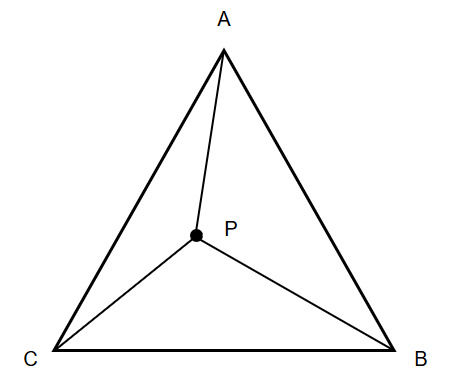
\includegraphics[scale=0.5]{images/barycentric_coordinates.jpg}
\caption{\label{img:barycentric_coordinates}Punkt $P$ im Dreieck $[ABC]$; Die Flächen der Dreiecke werden zur Bestimmung der barycentrischen Koordinaten genutzt}
\end{figure}

Die barycentrische Interpolation erlaubt die Interpolation zwischen drei Punkten auf einer Ebene, wobei die bekannten Punkte Eckpunkte eines Dreiecks darstellen. Die Interpolation wird mithilfe der barycentrischen Koordinaten durchgeführt. 

Die barycentrischen Koordinaten eines Punktes $P$ auf der Ebene sind ein Tripel aus reellen Zahlen $P = (x_P, y_P, z_P)$ \cite[vgl.][S. 6]{barycoords} und geben die Position eines Punktes relativ zu einem gegebenen Dreieck an. Die barycentrischen Koordinaten des Punktes $P$, bei dem gegebenen Dreieck $[ABC]$ (vgl. Abbildung \ref{img:barycentric_coordinates}), werden für den Fall, dass sich $P$ im Dreieck befindet, durch folgende Werte bestimmt:
\begin{align*}
x_P &= \frac{A_{[PBC]}}{A_{[ABC]}}\\
y_P &= \frac{A_{[PAC]}}{A_{[ABC]}}\\
z_P &= \frac{A_{[PAB]}}{A_{[ABC]}}
\end{align*}

Um barycentrische Koordinaten zur Interpolation zu nutzen soll folgende Situation betrachtet werden: Gegeben sei ein Punkt $Q$ mit den barycentrischen Koordinaten $(x_Q, y_Q, z_Q)$ und das Dreieck $[ABC]$. Die Punkte $A$, $B$ und $C$ haben jeweils einen zugewiesenen Wert $w$. Soll nun der Wert $w_Q$ am Punkt $Q$ durch barycentrische Interpolation der Werte $w_A$, $w_B$ und $w_C$ bestimmt werden, erfolgt die Berechnung von $w_Q$ folgendermaßen:
$$
w_Q = x_Q \cdot w_A + y_Q \cdot w_B + z_Q \cdot w_C
$$
Der Wert eines Eckpunktes des Dreiecks wird mit der barycentrischen Koordinate multipliziert, welche das Verhältnis der dem Punkt gegenüberliegenden Fläche zur Gesamtfläche des Dreiecks darstellt. Das heißt: Je näher der Punkt $Q$ an diesem Eckpunkt liegt, desto mehr wird der Wert dieses Eckpunktes gewichtet. Dies entspricht dem erwarteten Verhalten einer linearen Interpolation.

Damit die barycentrische Interpolation auf eine zufällig verteilte Punktewolke angewandt werden kann muss zunächst eine Triangulation für diese Punktewolke durchgeführt werden. Erst dann besteht die zu interpolierende Fläche nur aus Dreiecken. Betrachtet man nun zusätzlich mögliche Rundungsfehler durch die Ungenauigkeit von Fließkommazahlen in Computern empfiehlt es sich eine DeLauney-Triangulation durchzuführen um zu flache Dreiecke im Ergebnis der Triangulation zu vermeiden. Ein zu flaches Dreieck könnte sonst eine Fläche von $0$ erhalten, wodurch die Interpolation in diesem Dreieck aufgrund einer Division durch $0$ unmöglich wird.

\section{Triangulation}
\label{Triangulation}
Triangulation bezeichnet den Prozess aus einer Menge von Punkten ein Dreiecksnetz zu erstellen. Die Punkte werden dabei so mit Linien miteinander verbunden, dass Dreiecke aufgespannt werden.

Bei der DeLauney-Triangulation handelt es sich um eine spezielle Form der Triangulation, bei der die Umkreisbedingung erfüllt ist. Die Umkreisbedingung ist genau dann erfüllt, wenn in dem Umkreis eines Dreiecks keine Punkte zu finden sind und auf dem Umkreis nur Punkte des Dreiecks liegen. Durch die Erfüllung dieser Bedingung erhalten die Dreiecke im Dreiecksnetz eine besondere Eigenschaft: Die Innenwinkel der Dreiecke werden maximiert beziehungsweise der kleinste Innenwinkel der Dreiecke wird maximiert. So werden besonders flache Dreiecke im Dreiecksnetz vermieden.

Es gibt mehrere Algorithmen zur Durchführung einer DeLaunay-Triangulation, hier sollen zwei von ihnen vorgestellt werden. Der simpelste Algorithmus ist der sogenannte Flip-Algorithmus. Bei dieser Vorgehensweise wird zunächst ein einfaches Dreiecksnetz ohne Erfüllung der Umkreisbedingung erstellt. Im Anschluss wird die Umkreisbedingung für alle Dreiecke einzeln geprüft. Enthält der Umkreis eines Dreiecks den nicht gemeinsamen Punkt eines benachbarten Dreiecks wird ein Flip mit beiden Dreiecken durchgeführt. Hierzu kann man beide Dreiecke zusammen als Rechteck betrachten, die gemeinsame Kante beider Dreiecke ist dann die Diagonale dieses Vierecks. Für den Flip entfernt man nun diese Diagonale und ersetzt sie durch die andere Diagonale des Vierecks (siehe Abbildung \ref{img:flip_algorithm}). Nun muss die Umkreisbedingung für die beiden neuen Dreiecke erneut geprüft werden. Der Flip-Algorithmus hat einen Rechenaufwand von $O(n^2)$ da unter Umständen alle anderen Dreiecke nach einem Flip geprüft werden müssen.

\begin{figure}
\centering
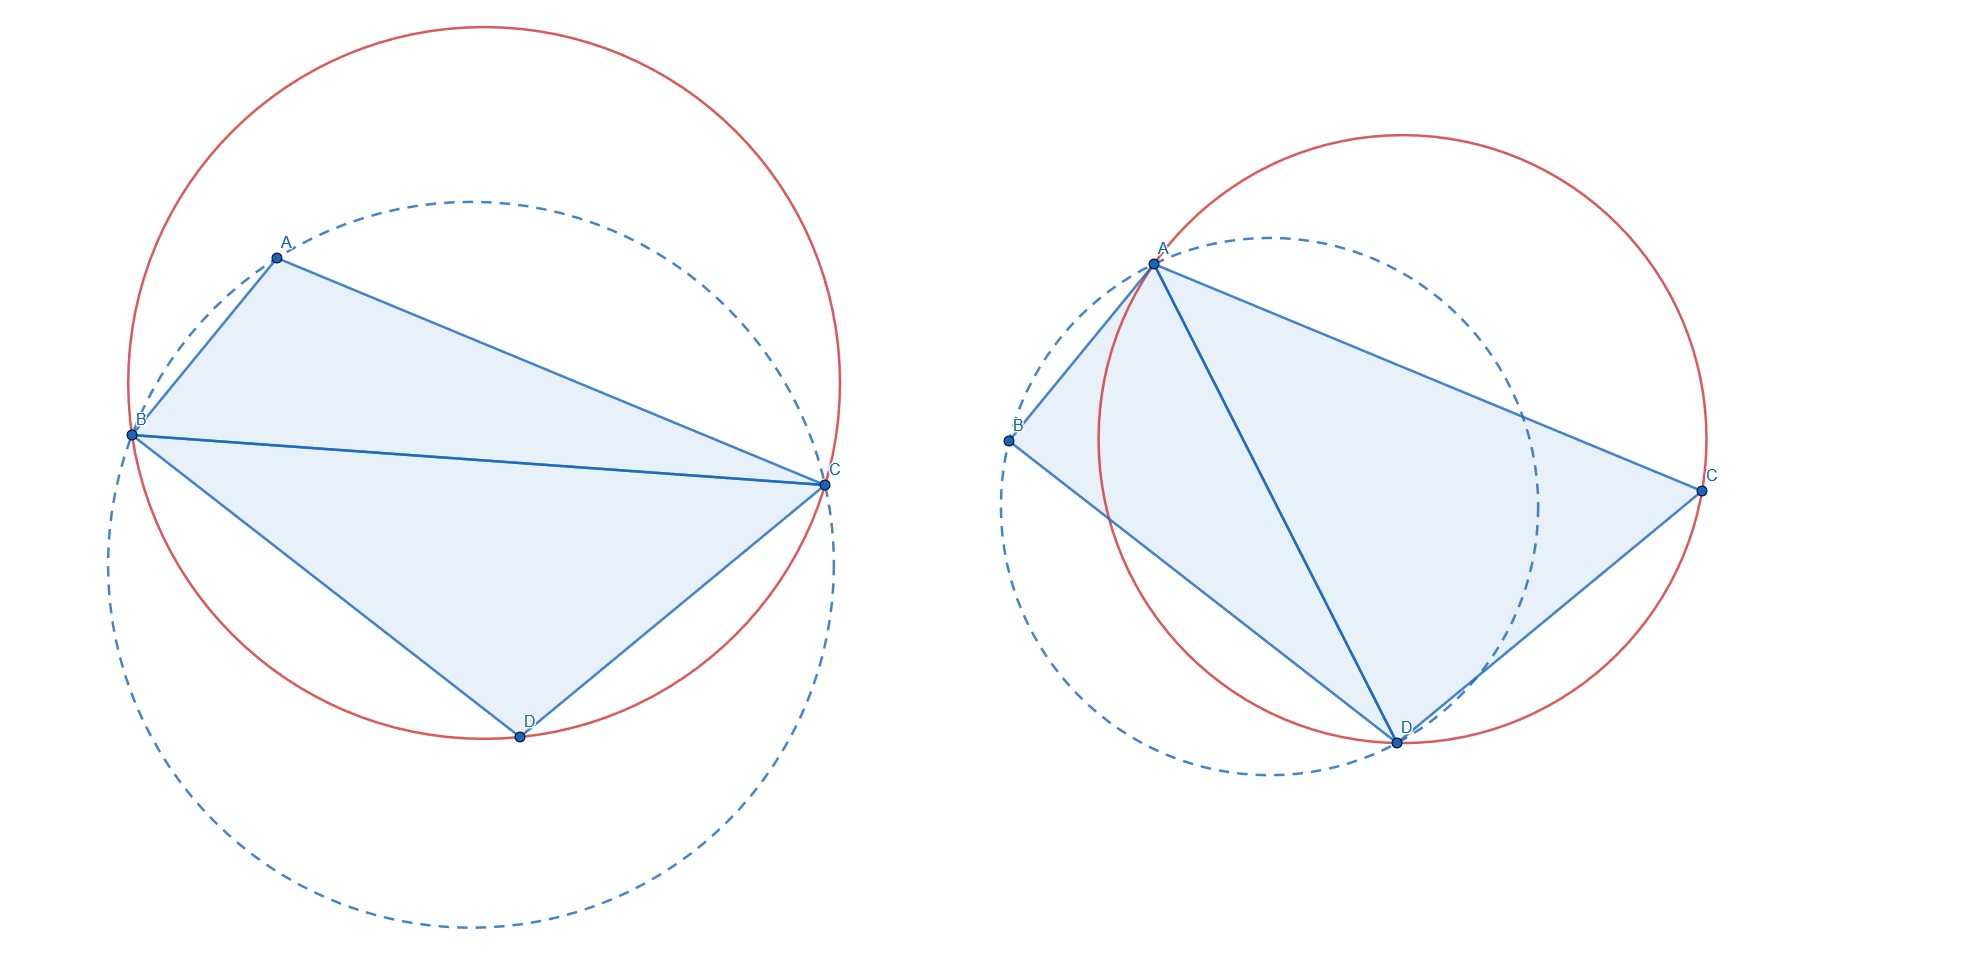
\includegraphics[scale=0.3]{images/flip_algorithm.jpg}
\caption{\label{img:flip_algorithm}Nach einem Flip wird die Umkreisbedingung für beide Dreiecke erfüllt}
\end{figure}

Der zweite Algorithmus ist eine Erweiterung des Flip-Algorithmus, welcher im Gegensatz zum reinen Flip-Algorithmus einen inkrementellen Ansatz verfolgt \cite[vgl.][S. 211ff]{computGeometry}. Hierbei werden die Punkte nacheinander hinzugefügt. Für diese Methode wird, bevor Punkte hinzugefügt werden, ein großes Dreieck benötigt, welches alle zu erwartenden Punkte einschließt. Nun kann damit begonnen werden die einzelnen Punkte hinzuzufügen. Wird ein Punkt eingefügt, muss das Dreieck bestimmt werden, welches den neu eingefügten Punkt enthält. Handelt es sich beim eingefügten Punkt um den ersten Punkt ist dies das große Dreieck, welches alle zu erwartenden Punkte einschließt. Ist das Dreieck, welches den neuen Punkt enthält, gefunden, werden drei Kanten von dem Punkt zu den Ecken des gefundenen Dreiecks gezogen, sodass dieses Dreieck in drei neue Dreiecke aufgeteilt wird. Diese neuen Dreiecke erfüllen noch nicht unbedingt die Umkreisbedingung, deshalb muss jedes einzelne nun auf diese geprüft werden. Bei Bedarf wird dann ein Flip durchgeführt, wodurch weitere Dreiecke geprüft werden müssen. Theoretisch ist der Aufwand für diese Korrektur $O(n)$. Es müssen allerdings nur in sehr seltenen Fällen alle Dreiecke korrigiert werden, weshalb ein Aufwand von $O(1)$ angenommen werden kann \cite[vgl.][S. 213]{computGeometry}. Der Gesamtaufwand der Inkrementellen Methode ist dann nur noch abhängig von der Effizienz der Suchmethode für das Dreieck, in welchem der neu hinzugefügte Punkt liegt. Einfache Suchansätze wie zum Beispiel einfaches Iterieren der Liste von Dreiecken haben einen Aufwand von $O(n^2)$ während eine Suche mithilfe einer Baumstruktur den Aufwand der gesamten Triangulation auf $O(n \log n)$ reduziert \cite[vgl.][S.213]{computGeometry}.

\section{Extrapolation}
Als Extrapolation bezeichnet man die Bestimmung von Werten, die außerhalb eines bekannten Wertebereiches liegen. Im Gegensatz zur Interpolation, bei der Werte zwischen zwei oder mehr anderen Werten bestimmt werden, werden bei der Extrapolation Werte außerhalb dieses Bereiches mithilfe bekannter Werte geschätzt.

Bei der Ausbreitung von Funkwellen können verschiedene Modelle angewandt werden, um die Empfangsfeldstärke in einer gewissen Distanz abzuschätzen, also zu extrapolieren. Diese Ausbreitungsmodelle können allerdings nicht immer oder nur mit vielen Informationen über die Umgebung genaue Schätzungen erzielen. Jedes dieser Modelle benötigt notwendigerweise die Entfernung zum Sender, um die Empfangsleistung zu bestimmen.

Das \textit{One Slope Model} ist eines der einfachsten empirischen Modelle zur Funkwellenausbreitung und benötigt keine Information über die Form des Raumes, in dem die Schätzung erfolgen soll. Es ist für den Indoor-Bereich konzipiert und macht die Dämpfung nur von der Entfernung zwischen Sender und Empfänger abhängig. Die Berechnung des Verlusts wird dabei folgendermaßen durchgeführt \cite[vgl.][S. 33]{markhoja}:
$$
L(d) = L_0 + 10\gamma\log d
$$
\begin{tabular}{ll}
$L$ & Verlustleistung [$dB$]\\
$L_0$ & Referenzverlustleistung bei $1m$ Entfernung [$dB$]\\
$\gamma$ & Verlustfaktor\\
$d$ & Entfernung zwischen Sender und Empfänger [$m$]
\end{tabular}
\\~\\
Der Verlustfaktor muss dabei für die vorraussichtliche Umgebungsbeschaffenheit empirisch bestimmt werden, um möglichst genaue Werte bei der Extrapolation zu erhalten. Je nach Umgebung kann sich der optimale Verlustfaktor durch günstige oder besonders ungünstige Reflexionen oder Absorptionen unterscheiden. Deshalb sind die Ergebnisse aus dem One Slope Model auch nur für grobe Näherungen geeignet und nicht zur genauen Berechnung von Empfangsfeldstärken.

Das \textit{Linear Attenuation Model} ähnelt dem One Slope Model sehr stark. Es unterscheidet sich insofern, als dass zur Berechnung zusätzlich die Freiraumdämpfung genutzt wird. Genauer wird die Freiraumdämpfung zusätzlich durch einen Faktor verstärkt um den zusätzlichen Verlust durch die Nutzung in Innenräumen zu berücksichtigen. Der Verlust an Empfangsleistung wird im Linear Attenuation Model folgendermaßen bestimmt \cite[vgl.][S. 33f]{markhoja}:
\newpage
$$
L(d) = F + ad
$$
\begin{tabular}{ll}
$L$ & Verlustleistung [$dB$]\\
$F$ & Freiraumdämpfung [$dB$]\\
$a$ & Dämpfungskoeffizient\\
$d$ & Entfernung zwischen Sender und Empfänger [$m$]
\end{tabular}
\\~\\
Auch hier muss ein Wert, nämlich der Dämpfungskoeffizient, empirisch bestimmt werden. Je nachdem, wie gut dieser Wert zu der Umgebung passt, in der die Verlustleistung bestimmt werden soll, desto genauer ist die Schätzung der Empfangsleistung. Aufgrund dieser Abhängigkeit von der Umgebung kann auch das Linear Attenuation Model nur für grobe Näherungen von Empfangsfeldstärken genutzt werden.

\section{Erweiterte Realität}

Unter Erweiterter Realität (auch augmentierte Realität; engl. Augmented Reality; abgekürzt AR) versteht man die Erweiterung der Realitätswahrnehmung durch virtuelle Objekte. Hierbei werden virtuelle Objekte, wie zum Beispiel Schilder, in die reale Welt in Echtzeit platziert (siehe Abbildung \ref{img:ar_signs}). Diese Objekte sollen dabei so gut an die Umgebung angepasst werden, dass sie wie echte Objekte wahrgenommen werden können.

Dies lässt sich durch verschiedene Techniken realisieren. Zunächst ist hier ein sogenanntes Head-Mounted-Display (HMD) zu nennen. Hierbei wird eine Art Brille mit einem vor den Augen montiertem Display genutzt, um dem Nutzer virtuelle Inhalte anzuzeigen. Für AR-Anwendungen muss dieses HMD entweder transparent sein oder das Bild einer Kamera für jedes Auge anzeigen, damit die Umgebung weiterhin wahrgenommen und nur augmentiert wird. Ist diese Transparenz nicht vorhanden spricht man von Virtueller Realität (VR). Dann werden nur virtuelle Inhalte angezeigt und der Nutzer sieht nichts mehr von seiner echten Umgebung.

Es gibt aber auch alternative Wege AR zu realisieren. So kann ein kleiner Display wie zum Beispiel ein Tablet oder ein Smartphone genutzt werden um ein \enquote{Fenster} in die augmentierte Welt zu erstellen. Das Display zeigt dabei das Kamerabild von einer (oder mehreren) Kameras hinter dem Display an und platziert virtuelle Objekte in diesem Kamerabild. Im Vergleich zu HMDs bietet dieser Ansatz weniger Immersion in die augmentierte Welt, benötigt allerdings keine zwei räumlich versetzte Bilder um ein realistisches 3D-Bild zu erstellen. Außerdem bietet sich diese Methode an, wenn eine möglichst große Nutzerzahl angestrebt wird, da viele bereits ein Smartphone oder Tablet (also einen Display mit einer Kamera auf der Rückseite) besitzen und somit keine neue Hardware für eine AR-Anwendung notwendig ist, vorrausgesetzt es ist ein Weg vorhanden, um die Position der Kamera zu verfolgen (Tracking).

\begin{figure}
\centering
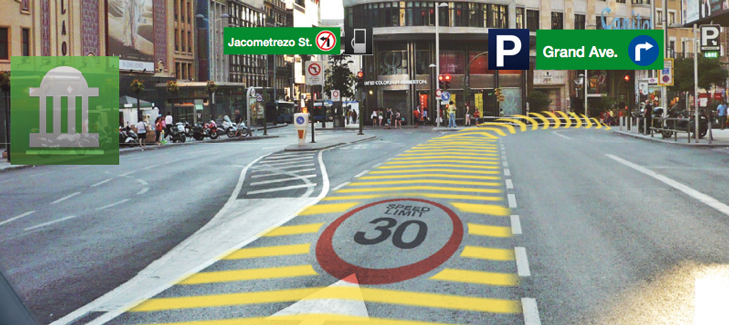
\includegraphics[scale=0.55]{images/ar_signs.jpg}
\caption{\label{img:ar_signs}In Augmented Reality können virtuelle Objekte in der echten Welt angezeigt werden. Bildquelle: \cite{arsigns}}
\end{figure}

\subsection{Inside-Out-Tracking}
Unter Inside-Out-Tracking versteht man im Kontext von augmentierter- oder virtueller Realität die Positionserkennung eines Gerätes ohne die Notwendigkeit von externer Hardware. Das Gerät nutzt in diesem Fall nur die ihm zur Verfügung stehenden Sensoren zur Erkennung seiner Position und darf nicht von in der Umgebung platzierten Geräten abhängen. Diese Art der Positionserkennung wird meist so realisiert, dass das Gerät mithilfe einer Kamera feste Punkte in der Umgebung sucht und aus der Bewegung dieser Fixpunkte Rückschlüsse auf die eigene Bewegung ziehen kann. Diese Fixpunkte sind dabei je nach System entweder vorher angebrachte Markierungen wie zum Beispiel QR-Codes oder gut unterscheidbare Punkte der Umgebung wie zum Beispiel die Kanten von Kacheln bei gefliestem Boden. 

\subsection{ARCore}
Bei ARCore handelt es sich um ein Framework von Google Inc. zur Erstellung von AR-Apps auf Android-Geräten. Einige Funktionen stehen hierbei auch für iOS zur Verfügung. ARCore ist der Nachfolger zu Google's \textit{Project Tango} und benötigt im Gegensatz zu seinem Vorgänger keine spezielle Hardware zur Entfernungsbestimmung im Kamerabild wie zum Beispiel eine ToF-Kamera\footnote{Bei einer ToF-Kamera handelt es sich um eine 3D-Kamera, die mit dem Laufzeitverfahren (engl. time of flight, kurz \textit{ToF}), also der Zeit, die ein Lichtblitz von der Kamera zur Szene und wieder zurück zur Kamera benötigt, Entfernungen bestimmen kann.} und unterstützt trotzdem weiterhin Inside-Out-Tracking.

ARCore stellt drei \cite{google2018} verschiedene Kernfunktionen zur Verfügung um das Erstellen von AR-Apps zu ermöglichen: Motion-Tracking um die Positionierung des Smartphones in Relation zu seiner Umgebung zu erlauben, Umgebungserkennung zum Erkennen und Verfolgen von Oberflächen, und Lichtestimation zur Anpassung der Beleuchtung von Virtuellen Objekten an die Beleuchtung der Umgebung.

\subsubsection{Bewegungserkennung}
Die Bewegungserkennung in ARCore verlässt sich auf zwei Datenquellen. Zunächst werden die Daten des Gyroskops und des Accelerometers ausgewertet, um eine Bewegungsvefolgung zu ermöglichen. Ein fundamentales Problem hierbei ist der sogenannte Drift, der aufgrund kleinster Fertigungsungenauigkeit, der Erdrotation, Vibrationen und anderen Faktoren zustande kommt. Durch den Drift wird die aus Gyroskop und Accelerometer berechnete (relative) Position zunehmend ungenauer. Dieser Drift wird in ARCore mithilfe der zweiten Datenquelle, dem Kamerabild, ausgeglichen \cite[vgl.][]{krempelarcoretango}. ARCore nutzt für die Auswertung des Kamerabilds den Prozess \enquote{concurrent odometry and mapping} \cite{arcoreconcepts2018}. Hierbei werden visuell unterscheidbare Fixpunkte genutzt, um eine verfolgbare Punktewolke zu erstellen. Mithilfe dieser Fixpunkte wird der Drift aus den Gyroskop- und Accelerometerwerten herausgerechnet und die genaue Position des Smartphones kann bestimmt werden.

\subsubsection{Umgebungserkennung}
Die Fixpunkte aus dem Kamerabild erlauben neben der Driftkorrektur außerdem die Umgebungserkennung. Durch Bewegung des Smartphones erhält ARCore unterschiedliche Perspektiven auf diese Fixpunkte, ähnlich wie mehrere Kameras. So kann bestimmt werden, welche Fixpunkte auf einer Ebene liegen. Befinden sich mehrere Fixpunkte auf einer Ebene kann ARCore auf diesen Ebenen Oberflächen vermuten. Auf diese Oberflächen sollen in AR-Anwendungen dann virtuelle Objekte platziert werden.

\subsubsection{Interaktion}
Die Interaktion mit AR-Umgebungen wird normalerweise durch Tracking eines gesonderten Eingabegeräts oder den Händen vorgenommen, damit der Nutzer die virtuellen Objekte \enquote{berühren} kann. Ein Smartphone eignet sich dafür nicht besonders gut, wenn es bereits als Fenster in diese Umgebung fungieren muss. Trotzdem sollen AR-Apps auf einem Smartphone eine Interaktion erlauben können. Neben statischen Knöpfen auf dem Smartphone-Display erlaubt ARCore deshalb außerdem das Antippen und Manipulieren (durch Gestensteuerung) von virtuellen Objekten. Dies wird so realisiert, dass Berührungen und Gesten auf dem Touchscreen an die Szene und Objekte in dieser weitergegeben werden, wenn diese Objekte auf dem Bildschirm die Position haben, auf der die Berührung oder die Geste ausgeführt wurde. Technisch wird dies durch einen Raycast von der Smartphone-Kamera in die dem Touch-Event entsprechende Richtung realisiert. Damit dieser Raycast in exakt die richtige Richtung ausgeführt wird müssen Eigneschaften der Kamera des Smartphones (zum Beispiel Position relativ zur Smartphone-Mitte, Brennweite der Linse und weitere) ARCore bekannt sein. Dies ist neben hohen Hardwareanforderungen einer der Hauptgründe, warum ARCore nur auf einer begrenzten Liste von Geräten verfügbar ist.

\subsubsection{Anchor}
ARCore korrigiert, während die App genutzt wird, laufend die Erkennung der Umgebung und Kameraposition. Damit virtuelle Objekte bei diesen Änderungen nicht ausgelassen werden nutzt man Ankerpunkte (engl. Anchor) um die virtuellen Objekte an eine Fläche zu binden. Korrigiert ARCore nach dem Platzieren eines Objekts die Fläche auf dem dieses steht, zum Beispiel indem der Winkel oder die Position geändert wird, dann wird das Objekt ebenfalls korrigiert. So bleiben Objekte immer am richtigen Punkt und ihre Position wird bei Bedarf mit der Fläche korrigiert.

\subsubsection{Persistenz}
Die Fixpunkte des Kamerabilds können, zumindest theoretisch, für das Persistieren der Positionierungsdaten genutzt werden, da die Fixpunkte immer wieder erkannt werden können, solange die Umgebung nicht zu stark verändert wird. Nur auf Gyroskop und Accelerometer gestütze Positionierungsverfahren können hingegen nur die Position relativ zum Startpunkt der Messung bestimmen.

In der Praxis bietet ARCore keinen Weg die Punktewolken lokal zu persistieren. Es gibt lediglich sogenannte Cloud-Anchor, die Ankerpunkte zwischen mehreren Geräten synchronisieren können. Diese Cloud-Anchor können allerdings nur zeitlich begrenzt (24 Stunden) gespeichert werden und sie funktionieren nur mit einer eigenen Google-Cloud Instanz \cite[vgl.][]{cloud2018}. Auf die (De\nobreakdash-)Serialisierungsmechanik für diese Cloud-Anchor hat man als Nutzer des ARCore-Framework keinen Zugriff. Deshalb ist ein Persistieren der Szene in der aktuellen Version von ARCore noch nicht für längere Zeit umsetzbar.

\section{Heatmap}
\begin{figure}
\centering
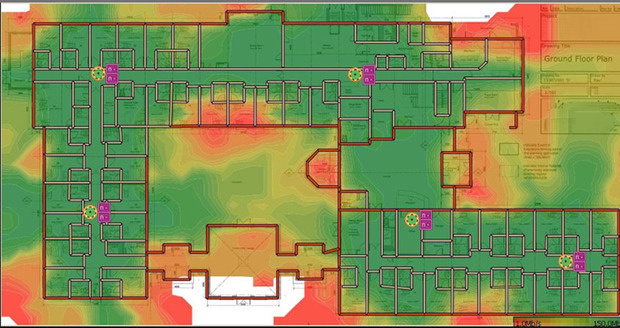
\includegraphics[scale=0.7]{images/wifi_heatmap.jpg}
\caption{\label{img:heatmap}Beispiel einer WLAN-Heatmap mit einem überlagerten Grundriss (Bildquelle: \cite{exheatmap})}
\end{figure}
Eine Heatmap stellt Funktionen mit einer eindimensionalen Zielmenge und einer zweidimensionalen Grundmenge dar. Beispiele für solche Funktionen wären Temperaturen an Orten, Höhendaten auf einer Landkarte oder WLAN-Empfangsstärken an einer Position in einem Haus (siehe auch Abbildung \ref{img:heatmap}). Es handelt sich also oft um ortsabhängige Messwerte. Die Zielmenge ist dabei auf einen bestimmten Zahlenbereich (zum Beispiel die Skala auf einem Thermometer) begrenzt, welcher dann auf einen Farbverlauf bezogen wird. Hierzu wird der Farbverlauf über die gesamte Breite des Bereiches gezeichnet, sodass jedem Wert im Bereich eine Farbe im Farbverlauf zugeordnet werden kann. Diese Zuordnung wird als Skala der Heatmap bezeichnet. Die Farben sollten hierbei so gewählt werden, dass sie eine Interpretation der Daten erlauben. Heatmaps für Temperaturen nutzen zum Beispiel häufig bläuliche Farben für kalte Umgebungen und die Farben rot oder weiß für heiße Umgebungen, da diese Farben normalerweise mit den entsprechenden Temperaturen in Verbindung gebracht werden. Bei Heatmaps für WLAN-Empfangsstärken hingegen ist grün für guten Empfang und rot für schlechten Empfang üblich.

\section{Anforderungsanalyse}
\subsection{Bestehende Lösungen}
Es gibt bereits viele Lösungen zur Analyse des eigenen WLAN. Die meisten von ihnen nutzen Heatmaps zur Visualisierung der WLAN-Empfangsstärke auf einer Karte oder einem Grundriss.

Zunächst sind hier professionelle Analysetools für PCs wie zum Beispiel \textit{Ekahau Site Survey} zu nennen, welches eine sehr detaillierte Analyse der WLAN-Verteilung erlaubt. Zur Vermessung des WLAN wird hier nicht der normale WLAN-Adapter des PCs verwendet, sondern spezielle Hardware, die die Analyse mehrerer Bänder und einzelner Frequenzen erlaubt und viele Störquellen eleminiert. Wird eine Messung mit dieser Software durchgeführt muss diese manuell auf einem importierten Grundriss platziert werden, um ihr einen Ort zuzuordnen.

Zur Analyse des WLAN-Netzes ohne teure Hardware sondern mit dem eigenen Smartphone existieren im \textit{Google Play Store} auch zahlreiche Apps. Die \textit{DSL Hilfe} App der Telekom oder die App \textit{WiFi Heatmap} erlauben zum Beispiel beide die Erstellung einer WLAN-Heatmap. Beide Apps verlangen hierzu das Zeichnen eines Grundrisses als Basis für die zu erstellende Übersicht. Im Anschluss werden Messungen mit der im Smartphone integrierten Antenne durchgeführt. Auch in diesen Apps muss die Messung dann manuell auf dem gezeichneten oder importierten Grundriss platziert werden.

\subsection{Erforderliche Anforderungen}
Die Android-App zur Vermessung und Visualisierung der Empfangsstärken soll in der Lage sein, die Position des Gerätes relativ zu seinem Startpunkt bestimmen zu können. Die Ortung muss dabei genauer als ein Meter sein, denn erst ab einer so hohen Genauigkeit ist die Positionierung genau genug, um mit manuellem Platzieren des Messpunktes auf einer Karte konkurrieren zu können. Die Ortung soll mithilfe des ARCore-Framework von Google realisiert werden. Dies sollte die mögliche Abweichung der Ortung weit unter einem Meter halten, da AR-Anwendungen bei kleinsten Abweichungen merkbare Darstellungsfehler bekommen, die den AR-Effekt mindern. ARCore muss deshalb in der Lage sein eine zentimetergenaue Ortung vorzunehmen.

Außerdem soll die App die Möglichkeit bieten, den Bereich in dem die Analyse durchgeführt werden soll, zu definieren. Dies soll nicht durch das Zeichnen eines Grundrisses dargestellt werden, sondern mithilfe von ARCore in AR geschehen. Die Begrenzungen des Bereiches sollen dabei mithilfe erweiterter Realität in die Umgebung gezeichnet werden. Wände und andere Objekte innerhalb des zu untersuchenden Bereichs müssen dabei nicht berücksichtigt werden.

Im Anschluss an die Bereichsdefinition soll die Vermessung des WLANs durchgeführt werden. Hierzu wird die empfangene Signalstärke aus dem Android-Betriebssystem ausgelesen. Die daraus resultierende RSSI-Messung soll zusätzlich eine Position erhalten. Diese soll mit der Position des Smartphones zum Zeitpunkt der Messung übereinstimmen. Zur Positionierung des Smartphones soll auch hier das ARCore-Framework genutzt werden.

Ist die Vermessung abgeschlossen, soll es in der App die Möglichkeit geben, eine Heatmap mit den RSSI-Werten zu erstellen und diese anschließend anzuzeigen. Die Heatmap ist dabei ein Bild, auf dem der Bereich vollständig abgebildet werden kann. Sie soll entweder eine relative Skala, deren Endpunkte durch den minimalen und maximalen gemessenen Wert definiert werden oder eine absolute Skala nutzen, welche sich an empfohlenen Empfangsstärken orientiert. Innerhalb des definierten Bereiches soll die WLAN-Empfangsstärke farblich gekennzeichnet werden, außerhalb soll das Bild transparente Pixel (Alpha-Kanal mit Wert 0) besitzen. Die Bereichsbegrenzungen selbst müssen dabei nicht gekennzeichnet werden, da die Grenze zwischen eingefärbten und transparenten Pixeln diese Grenze darstellt. Weiterhin sollen durch Interpolation die Lücken zwischen den Messwerten geschlossen werden, um eine durchgängige Heatmap zeichen zu können. Punkte, die nicht durch Interpolation berechnet werden, jedoch trotzdem im Bereich liegen, sollen den Wert des nächsten Messpunkts annehmen können. Zuletzt soll die Heatmap gespeichert werden können, um einen Vergleich mehrerer Messungen zu ermöglichen.

\subsection{Optionale Anforderungen}
Heatmaps können unterschiedlich gestaltet werden. Für die Farbgebung von Heatmaps werden meist ein paar Farben (Grundfarben) gewählt und zwischen ihnen ein Farbverlauf generiert. Um unterschiedliche Analysen zu ermöglichen, kann die Breite dieser Farbverläufe und der Grundfarben auf der Skala anpassbar gestaltet werden. Bei einem sehr schmalen Farbverlauf und breiten Grundfarben werden dann unterschiedliche \enquote{Zonen} markiert, die sich durch einen Bereich an RSSI-Werten definieren. Bei einem breiten Farbverlauf mit schmalen Grundfarben hingegen wird ein gleichmäßiger Farbverlauf auf der Heatmap erstellt. Für großflächige Analysen kann es von Vorteil sein, wenn die Auflösung der Heatmap selbst ebenfalls verstellt werden kann. So kann die Dateigröße bei besonders großflächigen Heatmaps klein gehalten werden, indem die Anzahl an Pixeln pro Meter verringert wird.

Für die Extrapolation von Messwerten kann eines der vorgestellten Ausbreitungsmodelle angewandt werden, um die ungefähre Empfangsstärke an nicht vermessenen und nicht interpolierbaren Orten abzuschätzen. Hierfür wird jedoch eine Technologie benötigt, mit der der Abstand zum Router bestimmt werden kann, wie zum Beispiel RTT des 802.11mc-Standards.

Je genauer die Ortung funktioniert, desto näher befindet sich die Heatmap an den tatsächlichen Maßen des Raumes. Bei Genauigkeiten unter 10 cm wird es möglich, die Heatmap in Augmented Reality anzuzeigen. So wird eine Visualisierung geboten, die potentielle Schwachstellen des Netzes direkt im Kamerabild markiert und nicht auf einer Karte anzeigt. Die Heatmap wird auf diese Weise begehbar gemacht.

\subsection{Abgrenzung}
Bei der in dieser Arbeit entwickelten App handelt es sich um einen Prototyp für ein Werkzeug zur Analyse von privaten WLAN-Netzen. Als Prototyp soll die App hauptsächlich demonstrieren, dass ein solches Werkzeug funktional in Form einer App realisiert werden kann. Die Bedienbarkeit der App wird dabei nur für Standardfälle berücksichtigt, sodass gewisse Randfälle einen Neustart der App erfordern können.

Das primäre Ziel des Prototyps ist zu demonstrieren, dass die Ortung eines Smartphones mithilfe des ARCore-Frameworks möglich ist. Außerdem soll demonstriert werden, wie AR als Eingabemethode genutzt werden kann, um Räume beziehungsweise Bereiche in eine digitale Form zu bringen, ohne dass ein manuelles Vermessen notwendig wird. Dies unterscheidet die in dieser Arbeit entwickelte Anwendung entscheidend von bereits vorhandenen Lösungen, die auf eine manuelle Positionierung von Messungen sowie auf das manuelle Anfertigen eines Grundrisses zurückgreifen.

\newpage

\section{Umsetzung}
Das gesamte AndroidStudio-Projekt der App zur Vermessung von WLAN-Empfangsstärken (\enquote{Wifi AR}), das Projekt für die Demo-App zum Testen der Funktionalität von Wifi RTT (\enquote{RTT Demo}) und eine digitale Version dieser Arbeit sind auf der beigelegten DVD gespeichert. Zusätzlich befinden sich auf der DVD drei Videos, mit denen die Funktionalität der App \enquote{Wifi AR} bei unterschiedlichen Einstellungen demonstriert wird.

Es gilt zu beachten, dass ARCore nur auf ausgewählten Android-Geräten installiert werden kann. Auf Geräten ohne offizielle ARCore-Unterstützung wird die App \enquote{Wifi AR} nicht funktionieren. Die App \enquote{RTT Demo} funktioniert nur auf Geräten mit mindestens Android 9.0 (Android P), die den WLAN Standard 802.11mc unterstützen.
\subsection{Entwicklungsumgebung}
\subsubsection{Software}
Bei dem in dieser Arbeit entwickelten Prototyp zur Vermessung von WLAN-Empfangsstärken handelt es sich um eine Android-App. Sie und die Demo-App \enquote{RTT Demo} wurden mithilfe der IDE \textit{Android Studio 3.1.3} entwickelt. Die Apps wurden komplett in der Programmiersprache Java geschrieben.

Für einige Tests war das Aufzeichnen des Smartphone-Bildschirms erforderlich. Hierzu kam die App \textit{AZ Screen Recorder} \cite{azrecorder} zum Einsatz.

\subsubsection{Hardware}
Für diese Arbeit wurde zunächst ein \textit{Google Pixel} und im Laufe der Arbeit dann ein \textit{Google Pixel 2} zur Verfügung gestellt. Beide Geräte waren jeweils mit einer Betaversion von Android 9 (Android P) als Betriebssystem ausgestattet.

Für die Messungen von RSSI-Werten und der generellen Funktionalität der App wurde mir eine \textit{FRITZ!Box 7590} von der AVM GmbH zur Verfügung gestellt. Für die Messungen der Distanzbestimmung mithilfe von WiFi RTT wurde dieser Router mit einer speziellen Firmware ausgestattet, die das Feature eingeschaltet hat.

\subsection{Benutzeroberfläche}
\label{UI}
\begin{figure}
\centering
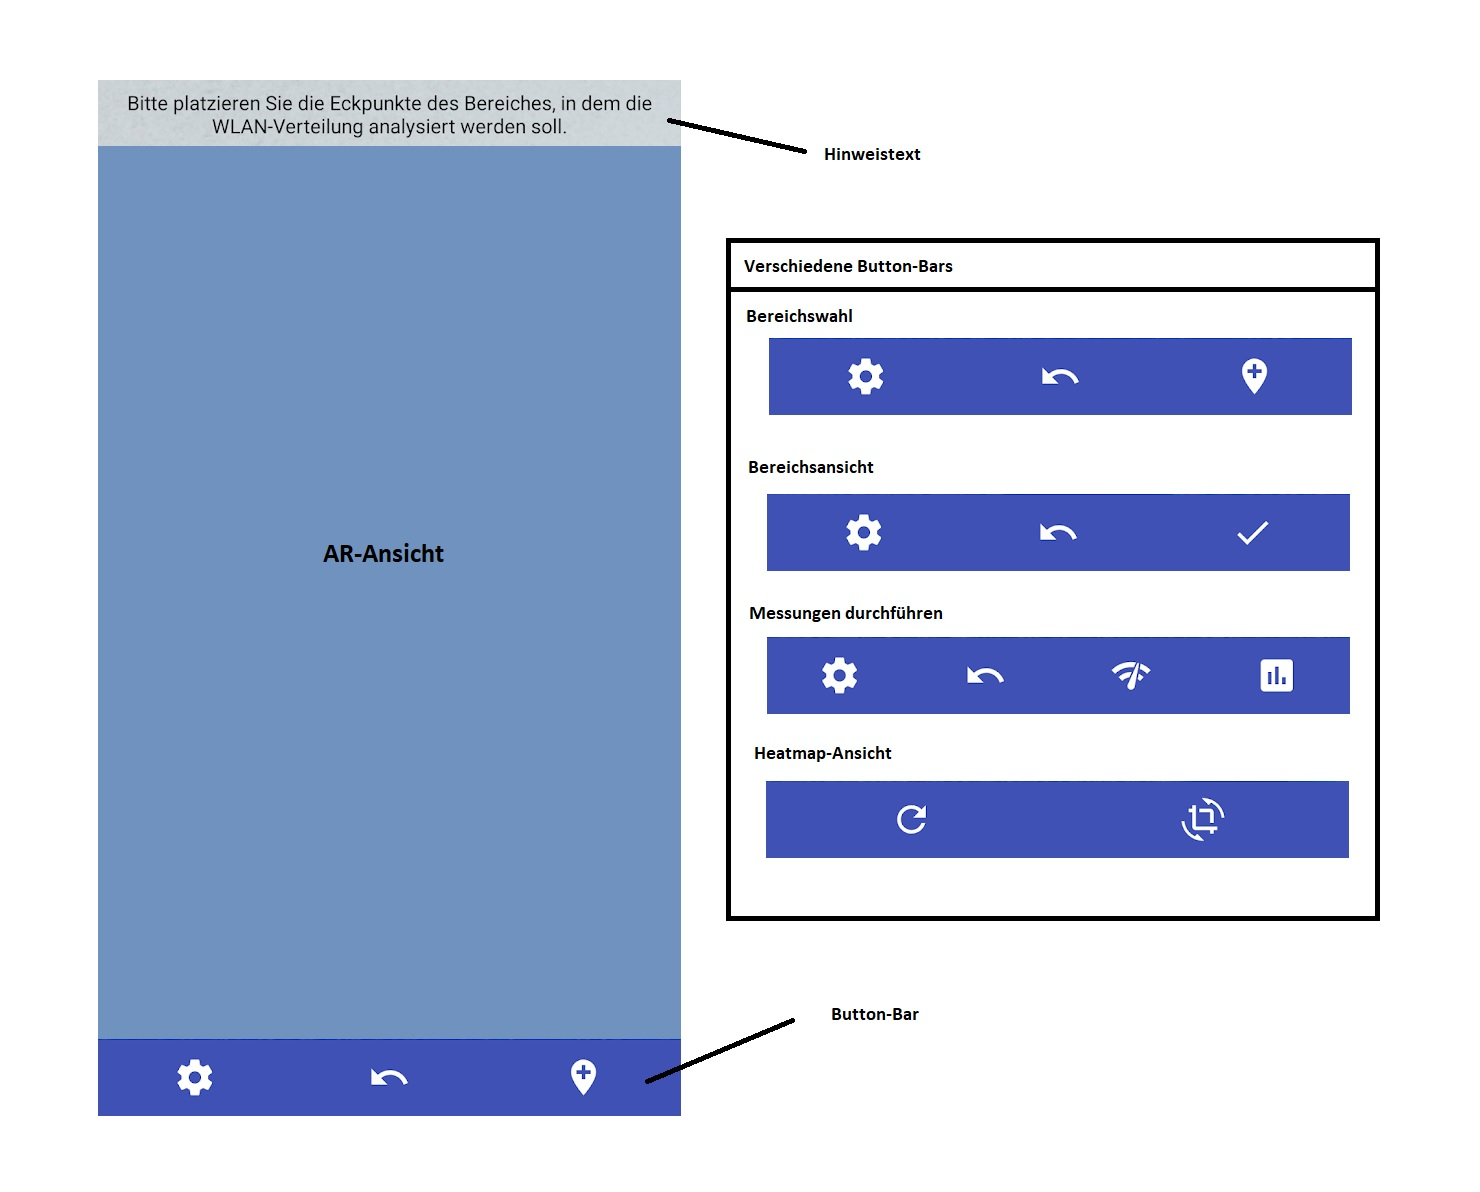
\includegraphics[scale=0.4]{images/ui.jpg}
\caption{\label{img:ui}Übersicht Benutzeroberfläche}
\end{figure}
Die Benutzeroberfläche der Hauptactivity\footnote{Die Hauptactivity der App ist die \textit{ArRecordVisualizeActivity}, siehe hierzu Kapitel \ref{MainActivity}} besteht aus drei wesentlichen Kernelementen. Das erste ist ein kleiner Hinweistext am oberen Bildschirmrand. Hier wird bis zur erstellten Heatmap immer ein kleiner Hinweistext angezeigt, der dem Nutzer vermittelt, was er momentan zu erledigen hat. An dieser Stelle wird auch der Fortschrittsbalken bei der Generierung von Heatmaps angezeigt.

Bei dem zweiten Element handelt es sich um die eigentliche AR-Fenster. Hier wird das aktuelle Kamerabild mit den Augmentationen angezeigt. Dieses Bildelement nimmt den meisten Platz auf der Oberfläche ein.

Das dritte Element ist eine Leiste mit Buttons, eine sogenannte Button-Bar. Die auf dieser Leiste verfügbaren Buttons werden je nach dem, in welcher Phase sich die App gerade befindet, geändert (siehe Abbildung \ref{img:ui} für alle möglichen Button-Bars). So werden nur momentan relevante Funktionen auf dem Bildschirm angezeigt und nicht unnötig viele Buttons.

Die Activity zum Speichern der Heatmap bietet neben dem natürlich notwendigen Button zum Speichern eine Aufsicht auf die erstellte Heatmap. Diese Aufsicht kann nach Bedarf mit einem Finger gedreht werden. So können Heatmaps in einer beliebigen Orientierung abgespeichert werden, um zum Beispiel das spätere Überlagern eines Grundrisses zu ermöglichen.

\subsection{AR-Umgebung}
Die AR-Umgebung wird mithilfe des \textit{ArFragment}s der Sceneform-Bibliothek bereitgestellt. Dies erlaubt eine einfache Initialisierung von ARCore und die Nutzung ohne OpenGL-Programmierung.

\subsection{Berechtigungen}
Das Android-Betriebssystem hat ein Berechtigungssystem, um unauthorisierten Zugriff auf potentiell sensible Resourcen zu verhindern. Der Nutzer muss diese Resourcen manuell freigeben. Die App benötigt für ARCore die Berechtigung zur Nutzung der Kamera. Die Abfrage dieser Berechtigung wird vom ArFragment beim Start der App übernommen. Für Zugriff auf die WLAN-Empfangsstärke wird Zugriff auf die Standortberechtigung erforderlich. Diese wird beim App-Start mithilfe der \textit{PermissionsDispatcher} API \cite{pdisp} abgefragt. Zuletzt benötigt die App Zugriff auf den internen Speicher des Smartphones zum Speichern der Heatmap. Diese Berechtigung wird mithilfe von \textit{PermissionsDispatcher} erfragt, sobald die erste Heatmap gespeichert wird.

\subsection{Bereichswahl}
\label{Bereichswahl}
\begin{figure}
\centering
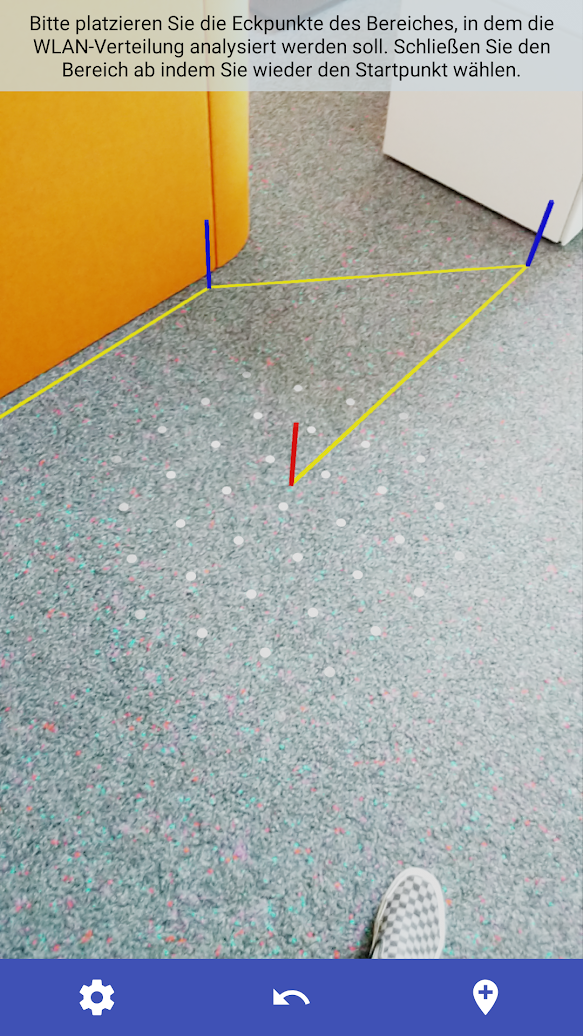
\includegraphics[scale=0.35]{images/bereichsdefinition.png}
\caption{\label{img:bereichsdefinition}Screenshot bei laufender Bereichsdefinition}
\end{figure}

Für die Erstellung der Heatmap ist es erforderlich, dass der zu analysierende Bereich zunächst eingegrenzt wird. So können einzelne Räume oder auch nur Teile von Räumen seperat analysiert werden. Außerdem wird durch die Begrenzung sichergestellt, dass wenn die Heatmap in AR dargestellt wird, diese nur an passenden Orten gezeichnet wird und nicht zum Beispiel außerhalb des Hauses weitergeht oder über Objekte verläuft. Wenn die Begrenzung entlang der Außenwände eines Raumes verläuft, kann diese Begrenzung sogar als Grundriss fungieren. Die Begrenzung soll durch ein Polygon festgelegt werden.

Die Bereichswahl kann auf mehrere Arten umgesetzt werden. So kann man die Eckpunkte des Bereiches zum Beispiel durch Antippen der entsprechenden Stellen im Kamerabild auf dem Display markieren. Dies würde jedoch durch die fehlende Präzision von Touch-Displays zu Ungenauigkeiten führen. Stattdessen wird eine Art Cursor entlang des Sichtvektors der Kamera genutzt. So können die Bereichspunkte präzise platziert werden. Optional kann die Bereichswahl mithilfe der Einstellung \enquote{Bereich automatisch definieren} ausgelassen werden. Dann wird der Bereich durch platzierte Messpunkte definiert.

Die Festlegung der Begrenzung erfolgt bereits in AR. Hierfür werden virtuelle, hohe Quader (wie quadratische Säulen) an den Eckpunkten des Bereiches aufgestellt (siehe Abbildung \ref{img:bereichsdefinition}). Diese Quader werden außerdem durch eine Linie Verbunden, damit die Ausmaße des designierten Bereiches sichtbar sind. Die Quader werden mithilfe der Sceneform-Bibliothek erstellt und platziert. Bei den Linien handelt es sich ebenfalls um Quader, allerdings mit einer sehr geringen Höhe. Auch die Linien werden daher mit der Quaderfunktion von Sceneform erstellt. Damit der Bereich und die Messpunkte später relativ zueinander platzierbar sind wird das Koordinatensystem von ARCore, welches sich dynamisch verändern kann, als gemeinsames Koordinatensystem genutzt. Aufgrund der potentiellen Veränderung im Koordinatensystem musste entschieden werden, ob die Eckpunkte des Bereiches je einen eigenen Anchor bekommen oder ob der gesamte Bereich an einen Anchor gebunden werden soll. Mehrere Anchor hätten den Vorteil, dass Eckpunkte garantiert an ihrer zugehörigen Stelle sind, wenn sie im Sichtfeld der Kamera sind. Allerdings kann die Form der Begrenzung so verändert werden, da Anchor unabhängig voneinander korrigiert werden können. Zusätzlich verbrauchen viele Anchor viel Rechenleistung, da jeder Anchor seperat überwacht und korrigiert werden muss. Wird der Bereich hingegen nur an einen Anchor gebunden bleiben die Form und die Maße des Bereiches garantiert gleich. Es kann in diesem Fall zu Ungenauigkeiten kommen, wenn der Anchor nicht im Bild ist (also nicht aktiv korrigiert wird), dies hat jedoch erst merkbare Auswirkungen sobald der Bereich besonders groß wird oder ARCore durch sehr radikale Bewegungen seine Referenzpunkte verliert (siehe hierzu Kapitel \ref{arcoreaccuracytest}).

In dem Prototyp wird der Bereich an nur einen Anchor gebunden, um den Rechenleistungsbedarf niedrig zu halten. Dieser eine Anchor liegt genau auf dem Startpunkt des Bereiches, also dem ersten Eckpunkt der platziert wird. Der Startpunkt setzt auch die Höhe aller folgenden Bereichspunkte fest, die Höhe der folgenden Punkte wird also auf die selbe Höhe korrigiert, auf der der Startpunkt des Bereiches liegt.

Die Eckpunkte des Bereichs werden in einem Stack organisiert, um dem Nutzer zu erlauben das Platzieren von Eckpunkten rückgängig zu machen. Die Logik zur Bereichsdefinition und die Verwaltung dieses Stacks wird durch die Klasse \textit{HeatmapGenerationController} übernommen.

Abhängig von der Einstellung \enquote{Bereich automatisch definieren} wird bei der Definition des Bereiches entweder mit dem Smartphone auf Eckpunkte gezeigt und diese gewählt oder der Nutzer führt direkt Messungen aus. In letzterem Fall wird der Bereich dann durch Messpunkte festgelegt. Das hat den Vorteil, dass keine Messungen mehr notwendig sind sobald ein Bereich definiert ist (weitere Messungen zur Verbesserung der Genauigkeit sind trotzdem möglich). Um die Platzierung von Messpunkten während der Bereichsdefinition zu vereinfachen, wird in diesem Modus der rote Cursor auf dem Boden unter dem Smartphone angezeigt.

\subsection{WLAN vermessen}
Nach der Definition des Bereiches beginnt die Vermessung des WLAN. Hierbei wird die WLAN-Empfangsfeldstärke aus dem Android-Betriebssystem mithilfe der Klasse \textit{WifiManager} ausgelesen. Hierfür wird die Berechtigung \inlcode{ACCESS\_COARSE\_LOCATION} (auf groben Standort zugreifen) benötigt, da eine App aus der WLAN-Umgebung Rückschlüsse auf den Standort des Nutzers ziehen kann. Wenn die Empfangsfeldstärke ausgelesen ist wird die Messung in der Einheit $mW$ anstatt $dBm$ gespeichert, um später nicht mit negativen Werten zu interpolieren. Das Auslesen der Empfangsstärke benötigt dabei, je nachdem, wie die entsprechenden Einstellungen gesetzt sind, ein wenig Zeit, um mögliche Fehler durch leicht zeitverzögerte Updates der Empfangsfeldstärke auszugleichen. Dieser Ausgleich wird durch simple Durchschnittsbildung zwischen zeitlich getrennten Einzelmessungen realisiert.

Als Position bekommt die Messung die Position der Kamera entlang der X- und Z-Achse des ARCore-Koordinatensystems und die Position entlang der Y-Achse (Höhe) wird aus dem Startpunkt des Messbereichs entnommen. So liegt der Messpunkt auf der gleichen Ebene wie der Bereich. Daraus folgt allerdings, dass die Höhe der Messung in dieser App nicht berücksichtigt wird, da die Verteilung auf eine zweidimensionale Darstellung projeziert werden soll. Die Analyse von mehreren Etagen ist somit nicht möglich. Potentielle Abweichungen, die durch Messungen auf unterschiedlichen Höhen zustande kommen können, werden durch die App nicht berücksichtigt, da diese auf einer zweidimensionalen Heatmap nicht dargestellt werden können.

Es ist zu beachten, dass Messpunkte auch außerhalb des Messbereiches liegen dürfen. Sie werden dann in die Berechnung der Heatmap mit einbezogen, liegen aber nicht in der erstellten Heatmap.

Ist die Einstellung \enquote{Bereich automatisch definieren} aktiviert beginnt der Ablauf in der App direkt mit der Erstellung von Messpunkten. Die ersten Messpunkte werden dann wie bei der normalen Bereichsdefinition durch Linien verbunden, um einen Bereich zu definieren. Der Bereich wird abgeschlossen, indem man sich wieder zum ersten Messpunkt begibt und dort auf \enquote{Messung durchführen} tippt sobald der rote Cursor auf den Startpunkt springt. Im Anschluss können noch weitere Messpunkte erstellt werden, die keinen Einfluss mehr auf die Form des Bereiches haben.


\subsection{Heatmap Generierung}
\subsubsection{Extrapolation}
\begin{figure}
\centering
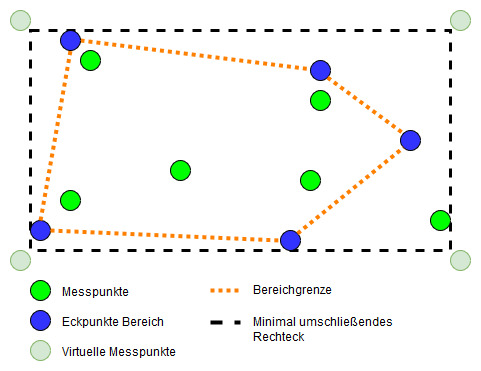
\includegraphics[width=0.6\textwidth]{images/ba_virtuelle_messpunkte.jpg}
\caption{\label{img:virtuelle_messpunkte}Skizze Virtuelle Messpunkte.}
\end{figure}
Interpolation kann nur innerhalb der konvexen Hülle des durch die Messpunkte definierten Polygons durchgeführt werden. Diese konvexe Hülle schließt nicht zwangsläufig den kompletten definierten Bereich ein, weshalb es Stellen in dem Bereich geben kann, deren Wert nicht durch Interpolation bestimmt werden kann. Deshalb wird zunächst das minimal umgebende Rechteck der Punkte des Bereiches und der Messpunkte bestimmt. Anschließend werden an den Eckpunkten dieses Rechtecks virtuelle Messpunkte erstellt (s. Abbildung \ref{img:virtuelle_messpunkte}).

Da der Wert dieser virtuellen Punkte nicht durch Interpolation bestimmt werden kann, muss hier eine andere Strategie angewandt werden. Optimalerweise müsste hier die Dämpfung der Empfangsfeldstärke vom nächsten Messpunkt aus berechnet und berücksichtigt werden, aber dies ist ohne bekannten Abstand zum Access Point nicht möglich. Eine solche Abstandsbestimmung wurde im Rahmen dieser Arbeit nicht realisiert, aber auf Umsetzbarkeit getestet (siehe Kapitel \ref{RTTTest}). Als Alternative bietet die App drei einfache Extrapolationsstrategien an: \inlcode{ASSUME\_LOW}, \inlcode{ASSUME\_HIGH} und \inlcode{ASSUME\_NEAREST}. Hierbei nehmen \inlcode{ASSUME\_LOW} und \inlcode{ASSUME\_HIGH} jeweils den tiefst- oder höchstmöglichen Wert an während \inlcode{ASSUME\_NEAREST} den Wert des nächsten Messpunkts annimmt. Die Strategien wurden aus Zeitgründen nicht in die Einstellungen der App übernommen, im Quellcode kann allerdings die genutzte Strategie festgelegt werden. Standardmäßig wird die Strategie \inlcode{ASSUME\_NEAREST} angewandt.

Wenn diese künstlichen Messpunkte den bestehenden hinzugefügt werden, liegen alle Punkte innerhalb des Bereiches auch garantiert innerhalb der konvexen Hülle des durch die Messpunkte definierten Polygons. Diese konvexe Hülle ist nun nämlich das durch die virtuellen Messpunkte aufgespannte Rechteck. So kann jedem Pixel der Heatmap nur durch Interpolation ein Wert zugewiesen werden.

\subsubsection{Interpolation}
Nicht für jeden Pixel in der Heatmap kann eine seperate Vermessung der WLAN-Empfangsstärke durchgeführt werden. Es gibt also deutlich weniger Messpunkte als Pixel in der Heatmap. Damit die resultierende Heatmap trotzdem keine Lücken hat, muss zwischen den Messpunkten interpoliert werden.

Für die Interpolation zwischen den Messpunkten wird in der App die barycentrische Interpolation (siehe Kapitel \ref{Interpolation}) angewandt. Damit diese jedoch genutzt werden kann, müssen die zu interpolierenden Punkte so verbunden werden, dass sie Dreiecke bilden. Um diesen Zustand zu erreichen, wird eine Triangulation zwischen den Punkten durchgeführt. Bei besonders flachen Dreiecken kann allerdings aufgrund der Ungenauigkeit von Fließkommazahlen die Berechnung der Fläche unmöglich werden. Die Fläche der Dreiecke wird jedoch bei der Interpolationsrechnung benötigt, weshalb flache Dreiecke vermieden werden sollten. Daher wird in der App die DeLauney-Triangulation verwendet, welche die Anzahl besonders flacher Dreiecke minimiert (siehe hierzu Kapitel \ref{Triangulation}). In der App wird die Triangulation mithilfe der Bibliothek \textit{DeLaunay-Triangulator} von Johannes Diemke \cite{jdi2015} durchgeführt. Die Bibliothek nimmt eine Menge an 2D-Vektoren als Eingabeparameter und gibt eine Sammlung von Dreiecken zurück. Dabei führt sie die Triangulation mithilfe des inkrementellen Flip-Algorithmus durch.

Ist die Triangulation abgeschlossen, beginnt die eigentliche Interpolation. Dabei wird jeder einzelne Pixel der Heatmap durchgegangen. Dies wird allerdings auf mehrere Threads aufgeteilt, um Nebenläufigkeit für diesen Prozess zu erlauben. Die Aufteilung ist dabei so realisiert, dass ein Thread nicht mehr als \inlcode{Constants.MAX\_VALUES\_PER\_THREAD} verschiedene Werte bearbeitet. Diese Konstante ist standardmäßig auf 10000 gesetzt. Beginnt die Bearbeitung eines Pixels, müssen zunächst den Eckpunkten des Dreieckes, in dem sich der Pixel befindet, die zugehörigen Messungen zugewiesen werden. Aufgrund der Nutzung einer Bibliothek für die Triangulation handelt es sich bei den Eckpunkten der Dreiecke nicht mehr notwendigerweise um Objekte von Typ \textit{WifiMeasurement}, sie können also nicht einfach wieder zu Messungen konvertiert werden. Stattdessen erfolgt die Zuweisung der Messungen zu den Eckpunkten eines Dreiecks sobald ein Pixel innerhalb eines Dreiecks bestimmt werden soll. Es werden dabei die Messungen mit den nächsten Koordinaten zu einem Eckpunkt für das entsprechende Dreieck ausgewählt. Die Messungen werden im Anschluss zusätzlich in einer \textit{HashMap} dem jeweiligen Dreieck zugewiesen, um den Zuweisungsprozess für alle folgenden Punkte in dem Dreieck zu verkürzen.

Sind die zugehörigen Messungen gefunden, wird für den den Pixel der Wert mithilfe von barycentrischer Interpolation und den Werten an den Messpunkten bestimmt. Ist der Wert für einen Pixel berechnet, wird dieser in eine Wertematrix (einen zweidimensionalen Double-Array) geschrieben. Dieser Prozess wird für jeden Pixel wiederholt. Hier ist zu beachten, dass bei der Generation der Wertematrix der ausgewählte Bereich noch nicht berücksichtigt wird. Jeder Pixel des minimal umschließenden Rechtecks der Messpunkte und der Bereichspunkte bekommt einen Wert zugewiesen.

\subsubsection{Farbgebung}
\label{Farbgebung}
Ist die Wertematrix generiert kann die eigentliche Heatmap erstellt werden. Hierfür werden zunächst die Farben aus den Einstellungen geladen. Die Farben werden dann äquidistant mit einer Farbe pro Pixel in einem Bild mit einer Höhe von einem Pixel und einer Breite von so vielen Pixeln wie in der Einstellung \enquote{Farbverlauf Breite} festgelegt (siehe Abbildung \ref{img:skala} für eine Visualisierung). Das bedeutet, der Pixel am linken Rand bekommt die Farbe, die den schlechtesten Wert repräsentiert und der Pixel am rechten Rand die Farbe, die den besten Wert repräsentiert. Alle anderen Farben werden so in dem Bild verteilt, das alle Farben die gleiche Entfernung in Pixeln zueinander haben. Die fehlenden Pixel werden mit einem Farbverlauf zwischen den Farben gefüllt. Dieses Bild ist die Skala für die Heatmap.

\begin{figure}
\centering
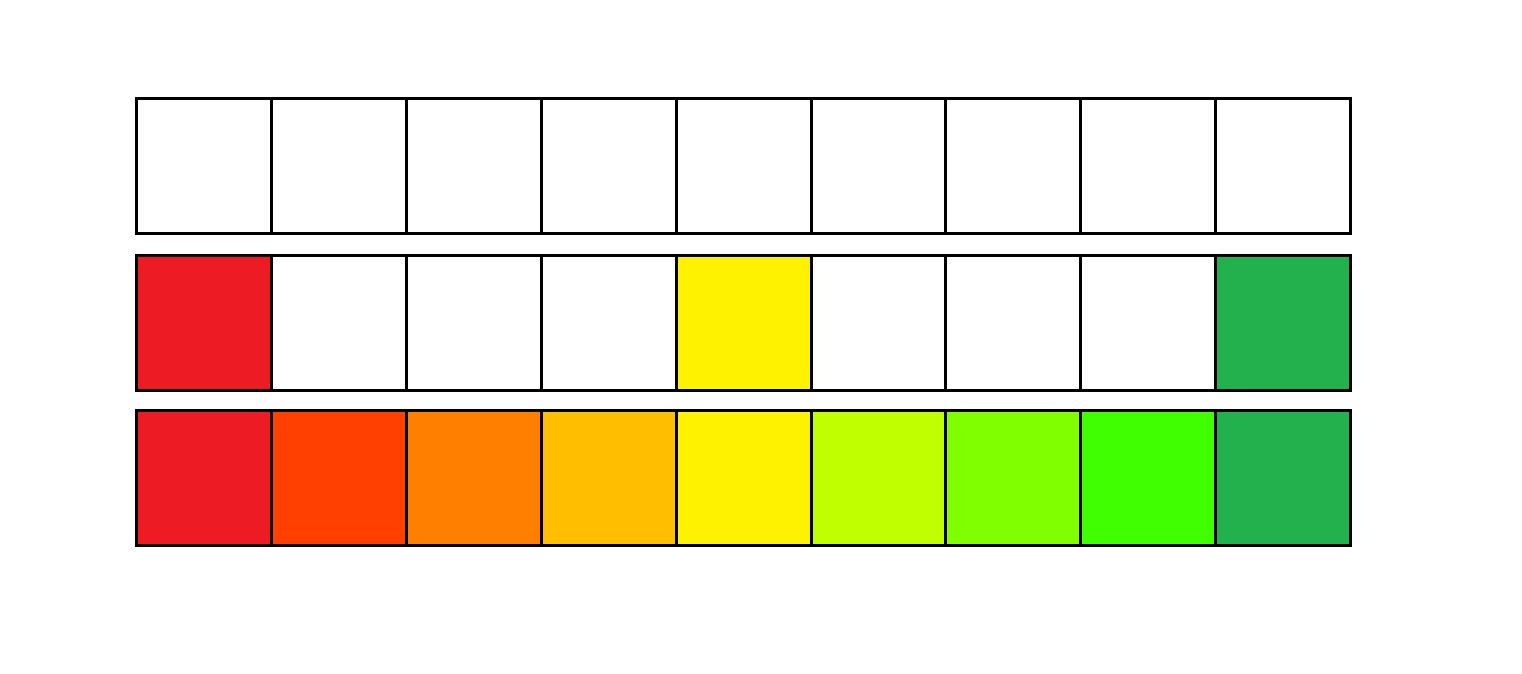
\includegraphics[scale=0.4]{images/skala.jpg}
\caption{\label{img:skala}Generieren der Skala mit einer Farbverlauf-Breite von 9 Pixeln}
\end{figure}

In einem zweiten Schritt werden die Grenzwerte festgelegt, also welcher Empfangsfeldstärken-Wert ist am besten und welcher am schlechtesten. Dies kann in dem Prototyp zum einen relativ bestimmt werden (also Minimum und Maximum des gewählten Bereiches in der Wertematrix werden als Grenzwerte gewählt). Alternativ erfolgt diese Grenzenwahl mithilfe der Android-SDK-Methode \inlcode{calculateSignalLevel(int rssi, int numLevels)} der Klasse \textit{WifiManager}. Dabei ist das niedrigste Level die Untergrenze und das höchste die Obergrenze. Bei letzterer Methode ist keine Wahl der Farbverlaufsbreite möglich, da die Methode nur eine feste Anzahl ganzzahliger Level liefert, deren Anzahl hier an der Anzahl der Farben festgelegt werden. Der Farbverlauf bekommt dementsprechend auch nur so viele Pixel an Breite, wie es Farben gibt. Die Wahl des Modus kann in den Einstellungen vorgenommen werden.

Nun werden für jeden einzelnen Pixel des Bereichs (Pixel außerhalb des Bereiches werden hierbei übersprungen) nacheinander die Farben bestimmt. Diese richten sich dabei danach, wo zwischen dem minimalen Grenzwert und maximalem Grenzwert der dem Pixel zugewiesene Wert liegt. Liegt der Wert zum Beispiel genau in der Mitte wird die Farbe gewählt, die sich in der Skala exakt in der Mitte befindet. Die entsprechende Farbe wird dann bei dem entsprechenden Pixel in der Ergebnis-Bitmap gesetzt.

\subsection{Einstellungen}
\begin{figure}
\centering
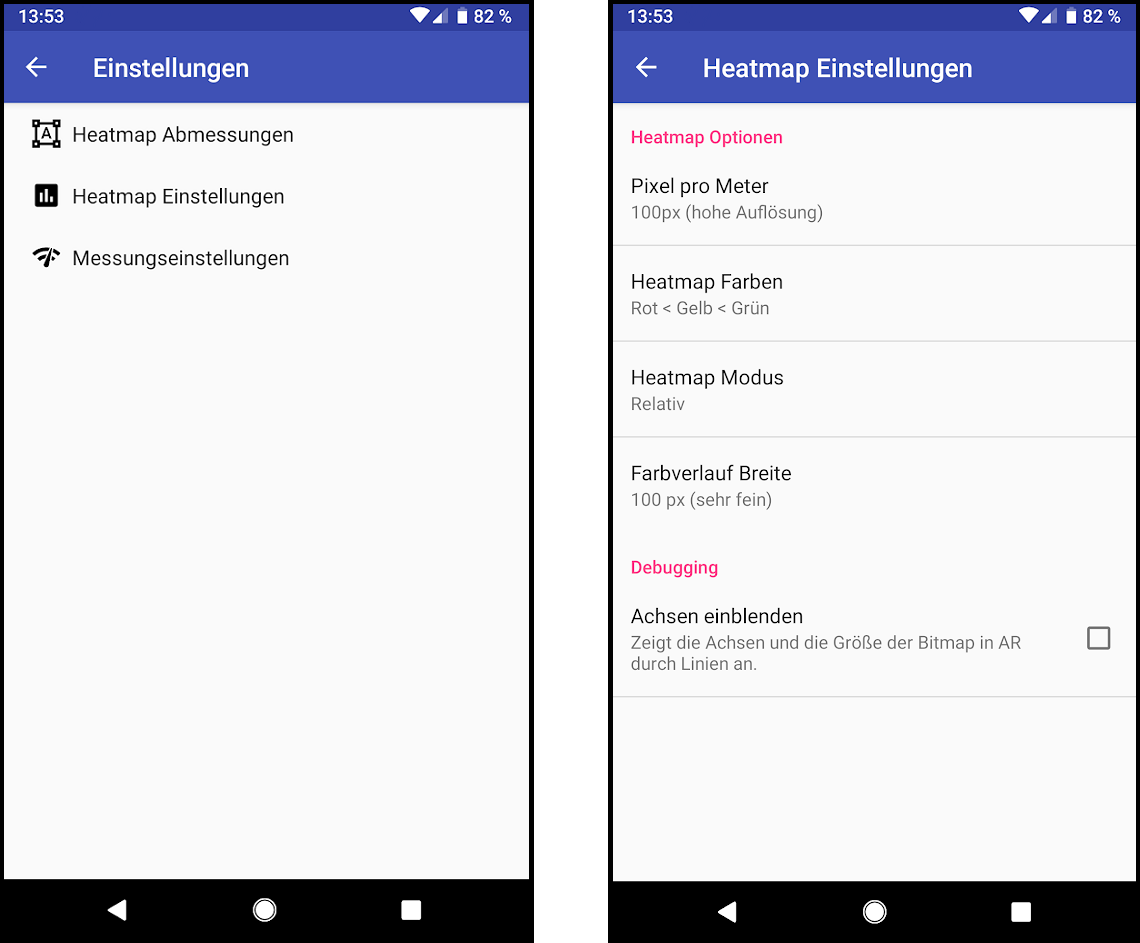
\includegraphics[scale=0.35]{images/einstellungen.png}
\caption{\label{img:einstellungen}Kategorien der Einstellungen (links) und Heatmap Einstellungen (rechts)}
\end{figure}

Die App bietet eine Reihe von Einstellungen um das Ergebnis und die Bedienung anzupassen. Diese sind mithilfe der Schaltfläche mit dem Zahnrad aufrufbar. Die Einstellungen werden mithilfe der \textit{SharedPreferences}-Klasse des Android-SDK persistiert, um einen Datenverlust bei App-Neustart zu vermeiden. Die Oberfläche der Einstellungen ist mithilfe der Klasse \textit{SettingsActivity} vom Typ \textit{PreferenceActivity} umgesetzt\footnote{Genauer ist die Klasse, welche die Einstellungen verwaltet (\textit{SettingsActivity}) eine Subklasse von \textit{AppCompatPreferenceActivity}, welche die \textit{PreferenceActivity} um Kompatibilitätsfunktionen erweitert.}. \textit{PreferenceActivity} erlaubt die Definition von Einstellungen mithilfe von XML-Dateien und kümmert sich um deren Persistenz.

Die Einstellungen sind in drei verschiedene Kategorien aufgeteilt (siehe Abbildung \ref{img:einstellungen}). In der Kategorie \enquote{Heatmap Abmessungen} befindet sich nur eine Einstellung, \enquote{Bereich automatisch definieren}. Diese Einstellung erlaubt es bereits in die Bereichsdefinition Messungen zu integrieren. Ist sie abgeschaltet, was sie standardmäßig ist, wird erst der Bereich für die Heatmap definiert und im Anschluss werden Messungen durchgeführt. Schaltet man diese Option hingegen ein, werden bereits bei der Bereichsdefinition Messungen durchgeführt.

In der Kategorie \enquote{Heatmap Einstellungen} werden sämtliche Einstellungen für das Generieren der Heatmap aufgeführt (siehe Abbildung \ref{img:einstellungen}). Hier kann die Auflösung der Heatmap (in Pixeln pro Meter), die Farben der Heatmap, der Modus der Heatmap und die Farbverlauf-Breite eingestellt werden. Beim Heatmap Modus kann entweder \enquote{Relativ} oder \enquote{Android Signal Level} ausgewählt werden. Im relativen Modus bekommt der schlechteste Wert der Wertematrix (der schlechteste Wert, der durch eine Farbe repräsentiert werden muss) die \enquote{schlechteste} Farbe und der beste Wert die \enquote{beste} Farbe. Der Modus \enquote{Android Signal Level} hingegen verlässt sich auf die Methode \inlcode{WifiManager.calculateSignalLevel(int rssi, int numLevels)}. Der RSSI-Wert an den Punkten wird mit dieser Methode in ein Signallevel umgewandelt, welches der Empfangsqualität entspricht (ähnlich der WLAN-Balken des Betriebssystems). Die Anzahl der möglichen Level ist dabei die Anzahl an eingestellten Farben. Da die Methode die RSSI-Werte in ganzzahlige Level umwandelt ist hier kein Farbverlauf möglich, weshalb die Option \enquote{Farbverlauf Breite} deaktiviert wird, wenn dieser Heatmap-Modus eingestellt ist. Es gilt zu beachten, dass der relative Modus nur die Verteilung des WLAN-Signals im untersuchten Bereich aufzeigen kann und keine Aussagekraft über die Qualität des Verbindungssignals hat. Bei dem Modus \enquote{Android Signal Level} handelt es sich hingegen um einen absoluten Modus, bei welchem die Farbe die Verbindungsqualität repräsentiert. In diesem Modus kann es dazu kommen, dass der gesamte untersuchte Bereich nur in einer Farbe eingefärbt wird, da alle Messwerte innerhalb eines Levels liegen.

Die Einstellung zur Farbverlaufsbreite legt fest, wie viele Pixel die Skala der Heatmap haben soll. Nähere Informationen hierzu sind im Kapitel \ref{Farbgebung} zur Farbgebung zu finden. Mit der Option \enquote{Achsen einblenden} können die Achsen von ARCore visualisiert werden. Ist diese Option eingeschaltet, wird das minimal umschließende Rechteck der Mess- und Bereichseckpunkte mithilfe von zwei Linien gekennzeichnet. Dieses Rechteck entspricht der Größe der Bitmap, auf der die Heatmap gezeichnet ist. Da es sich um das minimal umgebende Rechteck handelt sind die beiden Linien jeweils parallel zur X- und Z-Achse des ARCore-Koordinatensystems.

Die dritte Einstellungskategorie behandelt die Einstellungen für RSSI-Messungen. In dieser Kategorie befindet sich die Einstellung wie oft pro Messpunkt gemessen werden soll. Die Messungen liegen dabei immer mindestens eine Sekunde auseinander. Außerdem kann in dieser Kategorie festgelegt werden, ob auf neue \textit{ScanResults}\footnote{Ergebnisse eines WLAN-Scans in Android} gewartet werden soll, bevor eine weitere Messung durchgeführt wird. Auf diese Weise kann sichergestellt werden, dass der gelesene RSSI-Wert aktuell ist, da dieser mit neuen ScanResults aktualisiert wird. Es gilt jedoch zu beachten, dass ab Android P nur vier Scans pro zwei Minuten möglich sind. Wird dieses Limit überschritten (was in dieser App nach spätestens vier Messpunkten der Fall ist), wird automatisch nicht mehr auf neue ScanResults gewartet. Diese Einstellung hat also nur einen sinnvollen Effekt auf Geräten mit einer Android-Version unter Android P.

\subsection{Bedienung}
\subsubsection{Allgemein}
\begin{figure}
\centering
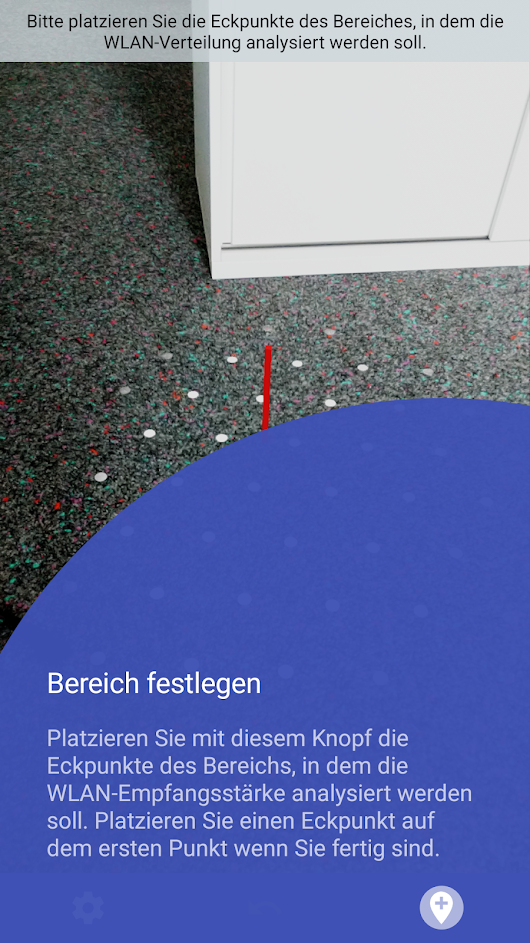
\includegraphics[scale=0.35]{images/tap_target.png}
\caption{\label{img:tap_target}Beispiel für ein Tap Target, hier für den Knopf zum Platzieren von Eckpunkten des Bereichs}
\end{figure}

Ziel war es, die Bedienung der App möglichst simpel zu halten, damit der Vorteil der App, nämlich das automatische Positionieren der Messungen, nicht durch eine komplizierte Bedienung verloren geht. Außerdem können nicht viele Bedienelemente platziert werden, damit genug Platz für das AR-Kamerabild bleibt. Wird dies zu klein kann der Nutzer Teile dieses Kernelements eventuell nicht mehr richtig erkennen. Das Layout der Oberfläche besteht daher nur aus einem Hinweistext, einer Leiste mit wenigen Knöpfen und dem Kamerabild (siehe auch Kapitel \ref{UI} für nähere Details zur Benutzeroberfläche). Mithilfe von \textit{Tap Targets} soll die Bedienung zusätzlich vereinfacht werden, indem der Nutzer beim ersten Öffnen der App durch die Kernfunktionen geleitet wird. Tap Targets heben eine Schaltfläche hervor und beschreiben ihre Funktion im Detail (für ein Beispiel siehe Abbildung \ref{img:tap_target}). Die App hat Tap Targets für die wesentlichen Kernfunktionen: Platzieren von Eckpunkten des Bereichs, Bereich abschließen, Messung durchführen und Heatmap generieren. Tap Targets werden nur einmal nach der Installation der App angezeigt. Sie sollen den Nutzer nur in die Bedienung einführen und nicht als dauerhafte Hilfe dienen. Hierfür wurde ein Hinweistext-Element am oberen Bildschirmrand platziert. Dieses zeigt immer an, wie der Nutzer jeweils vorzugehen hat.

Die Einstellung \enquote{Bereich automatisch erkennen} wurde nach dem Erstellen dieser Hilfestellungen hinzugefügt. Aus Zeitgründen war es nicht möglich, diese perfekt auf die Einstellung anzupassen, deshalb kann der Hinweistext am oberen Bildschirmrand hier unter Umständen nicht ganz stimmen und Tap Targets werden deaktiviert, wenn diese Einstellung aktiv ist.

\subsubsection{Anleitung}
Für die folgende Anleitung wird angenommen, dass die Einstellung \enquote{Bereich automatisch definieren} nicht verändert wurde, also abgeschaltet ist. Wird die App zum ersten Mal gestartet werden unter Umständen an einigen Punkten Tipps in Form von Tap Targets angezeigt. Diese lassen sich durch einen einfachen Klick irgendwo auf den Display oder durch das Ausführen der hervorgehobenen Funktion schließen.

Wird die App gestartet, muss zunächst das Tracking von ARCore genug Fixpunkte erkennen, um mit der Positionierung des Smartphones zu beginnen. Hierzu reichen langsame Drehbewegungen mit dem Smartphone aus. Wenn diese Kalibrierungsphase überwunden ist, verschwindet die entsprechende Animation über dem Bild.

Nachdem ARCore das Tracking aufgenommen hat, beginnt die Bereichsdefinition. Hierzu wird dort, wo man mit dem Smartphone hinzeigt, eine kleine rote Säule angezeigt. Diese fungiert als Cursor um die momentan anvisierte Position zu visualisieren. Nun wird der Bereich ausgewählt, in dem die WLAN-Empfangsfeldstärke angezeigt werden soll. Hierzu muss mit dem roten Cursor auf einen Eckpunkt des Bereiches gezielt werden und der Button ganz rechts (\enquote{Bereichspunkt hinzufügen}) auf der unteren blauen Leiste (Button-Bar) gedrückt werden. Die Eckpunkte werden dann mit einer blauen Säule markiert und die Bereichsgrenzen mit einer gelben Linie. Dieser Prozess soll dann für alle Eckpunkte des Bereiches wiederholt werden. Der Bereich wird abgeschlossen, indem auf den ersten Eckpunkt gezielt wird und dort der \enquote{Bereichspunkt hinzufügen}-Button betätigt wird. Der Bereich ist nun abgeschlossen und kann noch einmal überprüft werden. Wurde ein Fehler gemacht, können die Eckpunkte mit dem mittleren Button schrittweise rückängig gemacht werden. Entspricht der Bereich den Vorstellungen, kann mit einem Klick auf den Button am rechten Rand der Button-Bar, der nun einen Haken anzeigen sollte, der Messungsmodus gestartet werden.

Im Messungsmodus können nun die WLAN-Empangsstärken an unterschiedlichen Orten gemessen werden. Hierzu stellt man sich jeweils an einen Ort und führt dort mit dem Button \enquote{WLAN messen} (der zweite Button von rechts) eine Messung durch. Wenn die Messung abgeschlossen ist wird an dem Ort, an dem die Messung vorgenommen wurde, eine grüne Säule platziert. Zur Erstellung einer Heatmap sind mindestens drei Messpunkte erforderlich, das Ergebnis verbessert sich allerdings deutlich durch mehr Messungen. Sind die gewünschten Messungen durchgeführt, kann die Heatmap mit einem Klick auf den Button \enquote{Heatmap generieren} (der rechteste Button) erstellt werden. Nach einer kurzen Ladezeit erscheint diese dann auf dem Boden und kann ausgewertet werden.

Soll die Heatmap geteilt werden, kann dies mit einem Klick auf den Button ganz rechts mit dem Symbol zur Rotation eines Bildes geschehen. Es öffnet sich eine Ansicht, in der die Heatmap nach Wunsch mit einem Finger rotiert und im Anschluss gespeichert werden kann. Die Heatmap kann dann in der Galerie des Geräts gefunden werden. Soll eine erneute Analyse durchgeführt werden, kann dies mit dem Button mit dem \enquote{Neu Laden}-Symbol (ein im Kreis zeigender Pfeil) neben dem Knopf zum Speichern der Heatmap getan werden.

\subsection{Klassen}
In diesem Kapitel sollen die wichtigsten Klassen kurz in ihrer Funktionalität beschrieben werden um einen Überblick über die Architektur der App zu geben.

\subsubsection{ArRecordVisualizeActivity}
\label{MainActivity}
Diese Klasse repräsentiert die zentrale Activity der App. Hier werden bei Bedarf Anfragen nach Berechtigungen erstellt, Views initialisiert, Klicks auf Schaltflächen empfangen und ein HeatmapGenerationController verwaltet. Die Klasse nimmt, in Bezug auf das MVC-Modell, eine Mischung aus Controller (Lifecycle-Management und Berechtigungsmanagement) und View (Führt UI-Änderungen aus, wie zum Beispiel am Hinweis-Text am oberen Bildschirmrand; Erhält onClick-Events auf den Buttons) als Rolle an. 

\subsubsection{HeatmapGenerationController}
In dieser Klasse liegt die Logik der Erstellung von Heatmaps. Die Klasse übernimmt das Festlegen des Bereichs, das Erstellen von Messpunkten und das Generieren der Heatmap. Methoden der Klasse werden von der ArRecordVisualizeActivity aufgerufen um bestimmte Aktionen wie beispielsweise \enquote{Neuen Messpunkt erstellen} auszuführen. Über das Interface \textit{HeatmapGenerationControllerCallback} können Callbacks für Statusänderungen und Visualisierungsinformationen des HeatmapGenerationControllers empfangen werden. In der App erhält die ArRecordVisualizeActivity diese Callbacks. Spezifische Funktionen werden an weitere Klassen wie zum Beispiel den \textit{HeatmapGenerator} delegiert.

\subsubsection{HeatmapGenerator}
Die Klasse HeatmapGenerator enthält die Logik zum Erstellen einer gefüllten Wertematrix aus einer Sammlung von Messpunkten. Hier wird die Delauney-Triangulation und die Interpolation durchgeführt. Die resultierende Wertematrix enthält für jede ganzzahlige Koordinate einen Wert, der anhand der gegebenen Messpunkte durch Interpolation oder eine \textit{ExternalPointStrategy} bestimmt wurde. Die interne Klasse \textit{ExternalPointStrategy} legt fest, wie Werte außerhalb der konvexen Hülle der Messpunkte bestimmt werden.

\subsubsection{BitmapGenerator}
Der BitmapGenerator soll aus einer Wertematrix eine Bitmap erstellen. Jeder Eintrag in der Wertematrix stellt dabei einen Pixel dar. Die Bitmap soll für jeden Pixel eine Farbe bekommen, die den Wert an dieser Stelle repräsentiert. Diese Umrechnung von Wert zu Farbe wird von dem im Konstruktor übergebenen ColorSelector übernommen, welcher wiederum je nach eingestelltem Modus und eingestellten Farben die Pixelfarbe für einen Wert auswählt.

\subsubsection{ColorSelector}
Diese Klasse übernimmt die Auswahl der Farbe für einen bestimmten Wert. Hier wird die Skala der Heatmap verwaltet. Der \textit{BitmapGenerator} entnimmt einem Objekt dieser Klasse die Farbe für einen Wert.

\subsubsection{DrawingHelper}
Die Hilfsklasse DrawingHelper stellt eine kleine Gruppe von statischen Hilfsmethoden zur Verfügung um in einer ARCore-Umgebung Marker und Linien zu zeichen.

\subsubsection{OnboardingHelper}
Der OnboardingHelper enthält einige Hilfsmethoden zum Anzeigen von spezifischen Tap Targets, wenn sie nicht bereits gezeigt wurden.

\subsubsection{Preferences}
Diese Klasse erlaubt das einfache Persistieren und Laden von primitiven Datentypen sowie das Laden von Einstellungen. Hierfür werden die SharedPreferences des Android SDK genutzt.

\subsubsection{Polygon}
Diese Klasse repräsentiert einen Bereich, der durch eine Reihe von Eckpunkten definiert wird. Sie bietet eine Methode um zu prüfen, ob ein Punkt in dem Bereich liegt. Diese Methode wird vom \textit{BitmapGenerator} genutzt, um zu bestimmen, ob ein Pixel eine Farbe für seinen Wert bekommt oder transparent sein soll (was der Fall ist wenn der Pixel außerhalb des definierten Bereiches liegt).

\subsubsection{RssiAggregate}
Diese Klasse dient dem Aggregieren von RSSI-Messwerten. Pro Punkt werden mehrere (so viele wie in den Einstellungen angegeben) Messungen durchgeführt. Ein Objekt der Klasse \textit{RssiAggregate} aggregiert dabei die Messwerte. Dies erlaubt die Bildung eines Durchschnitts.

\subsubsection{WifiMeasurement}
Diese Klasse repräsentiert einen Messpunkt. Sie enthält den gemessenen RSSI-Wert, die Wellenlänge des gemessenen WLAN-Signals sowie die Position der Messung.

\subsubsection{ArWifiToolbar}
Bei der \textit{ArWifiToolbar} handelt es sich um die Button-Bar am unteren Bildschirmrand der \textit{ArRecordVisualizeActivity}. Sie führt alle notwendigen UI-Operationen aus, damit die Toolbar zu der aktuellen Phase der App passt.

\subsubsection{WifiDataCollector}
Die Klasse \textit{WifiDataCollector} erlaubt den Zugriff auf Daten über die WLAN-Verbindung des Smartphones wie zum Beispiel den RSSI durch Hilfsmethoden, die Einheitenumrechnug verbergen. Außerdem bietet die Klasse die Möglichkeit per Listener-Interface (\textit{ScanResultsAvailableListener}) über neue ScanResults informiert zu werden.

\subsection{RTT Demo App}
\label{rttapp}
Neben der App \textit{Wifi AR} zum Vermessen und Visualisieren von WLAN-Empfangsstärken wurde im Rahmen dieser Arbeit eine kleine Demo App geschrieben, mit welcher die Abstandsmessung zu APs mit dem RTT-Verfahren (siehe Kapitel \ref{rtt}) getestet werden kann. Mit dieser App sollte evaluiert werden, wie genau das Verfahren auf bestehender Hardware funktioniert und inwiefern sich die gemessene Distanz zur Nutzung bei der Extrapolation von Messwerten eignet (siehe Kapitel \ref{RTTTest}). Die App besitzt dabei nur einen einzelen Button mit der Beschriftung \enquote{START}. Drückt man diesen Knopf, erhält man nach kurzer Wartezeit darunter eine Liste mit den RTT-Ergebnissen. Dabei gilt zu beachten, dass auf Android Geräten nur begrenzt viele RTT-Anfragen gleichzeitig (10 auf dem \textit{Google Pixel 2}) durchgeführt werden können. Deshalb können nicht alle APs in Reichweite getestet werden. Aus diesem Grund nutzt die App die Methode \inlcode{ScanResult.is80211mcResponder()} bei den einzelnen ScanResults, um APs mit Unterstützung für RTT zu priorisieren. So wird verhindert, dass nur APs ohne RTT Unterstützung in den Ergebnissen landen.

\newpage

\section{Untersuchungen}
Zur Untersuchung der in dieser Arbeit erstellten App wurden einige Messungen durchgeführt. Diese Messungen sollen bestimmen, wie hilfreich das erstellte Tool sein kann und wo dessen Grenzen liegen.

Die Tests wurden auf einer WLAN Teststrecke der AVM GmbH durchgeführt (siehe Abbildung \ref{img:wlan_loft}). Diese befindet sich weitab von vielen WLAN Netzen, daher werden hier Störeinflüsse minimiert. Gleichzeitig befindet sich die Teststrecke in einem Gebäude, um die WLAN-Umgebung in einer Wohnung oder einem Haus zu simulieren. Sie bietet außerdem eine gleichmäßige Beleuchtung und farblich unterscheidbare Raumelemente, also eine günstige Umgebung zur optischen Fixpunkterkennung.

\begin{figure}
\centering
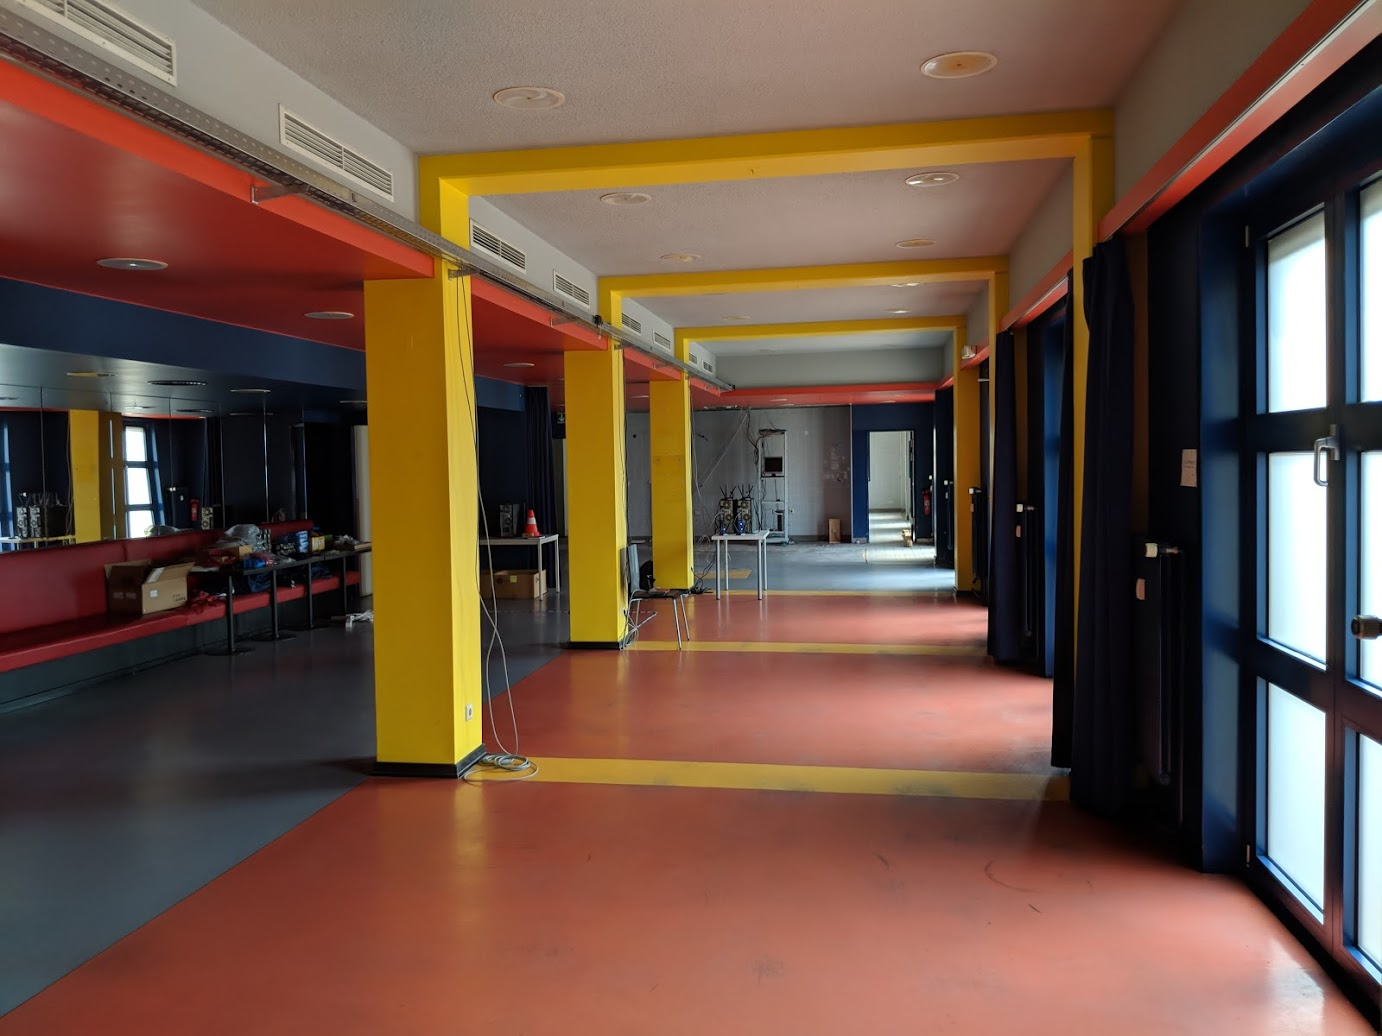
\includegraphics[scale=0.25]{images/wlan_loft.jpg}
\caption{\label{img:wlan_loft}WLAN-Teststrecke der AVM GmbH}
\end{figure}

Für jeden Test wurde in der App die schnelle Messmethode (ohne Warten auf neue ScanResults) angewandt. Als Anzahl an Messungen pro Messpunkt wurde auf $5$ festgelegt. Deshalb handelt es sich bei jeder angegebenen RSSI-Messung um einen Durchschnittswert von $5$ unterschiedlichen Messungen. Als Testgerät diente ein \textit{Google Pixel 2}, viele Ergebnisse sind aufgrund von starken Hardwareunterschieden zwischen Android-Smartphones nur bedingt auf andere Geräte übertragbar. Als AP für die Tests wurde eine \textit{FRITZ!Box 7590} verwendet.

\subsection{Reproduzierbarkeit von Empangsfeldstärken-Messungen}
\label{reproductability}
Im Folgenden wurde die Reproduzierbarkeit von Messungen der WLAN-Empfangsfeldstärke untersucht. Hierzu wurde zunächst eine Position in drei Meter Entfernung von einem WLAN-Router (welcher sich auf dem Boden befand) markiert. Im Anschluss daran wurde in der App ein beliebiger Bereich definiert, die Größe und Position des Bereiches waren für diesen Test nicht relevant. Dann wurde an der markierten Position eine WLAN Messung mithilfe der App durchgeführt. Um das Szenario einer echten Messung für die App zu simulieren, wurde das Smartphone zwischen den einzelnen Messungen kurz 10 Meter von dem Messpunkt entfernt, um im Anschluss wieder auf den Messpunkt bewegt zu werden. Außerdem wurde das Smartphone stets mit der Kamera senkrecht Richtung Boden gehalten und es wurde dafür gesorgt, dass das Smartphone LOS zum AP hat. Am Ende einer Messung zeigt die App den gemessenen RSSI-Wert mithilfe eines Toasts an. Diese Anzeige wurde hier zur Auswertung der Messungen genutzt.

In Tabelle \ref{tab:rssiReproduction} können die Messergebnisse am gleichen Punkt im drei Metern Entfernung vom Router eingesehen werden. Die Messergebnisse schwankten dabei in einem Bereich von $6,36$ dBm, hatten jedoch eine Standardabweichung von $1,478$ dBm. Diese Abweichung ist gering genug, dass Bereiche mit schlechtem Empfang auch als solche erkannt werden können. Für den Fall, dass sich die Farbskala der Heatmap im relativen Modus befindet, ist zu berachten, dass es in kleineren Messbereichen zu widersprüchlichen Ergebnissen kommen kann. Ein solcher Effekt wurde bei den Tests zur Genauigkeit der Interpolation (siehe kapitel \ref{InterpolationAccuracy}) in Bereichen mit $1\cdot 1$ m Grundfläche beobachtet, trat ab $2\cdot 2$ m Grundfläche allerdings nicht mehr auf.
Unter Umständen ist die mögliche Abweichung groß genug, dass sie die Auswertung der Ergebnisse anderer Tests zur RSSI-Messung erschweren kann. Differenzen von weniger als $1,478$ dBm, aber auch zwischen $1,478$ dBm und $6,36$ dBm, können sowohl durch die Änderung eines Parameters hinzugekommen sein als auch durch die mäßige Reproduzierbarkeit von Messungen. Solche Abweichungen können also nur sehr bedingt auf die zu testenden Parameter zurückgeführt werden.

\begin{table}
\centering
\begin{tabular}{|r|r|r|r|}
\hline
Messung & RSSI & Abweichung & Quadr. Abweichung\\
Nr. & $[dBm]$ & vom Mittelwert & vom Mittelwert \\\hline
1 & -48,38 & 1,368 & 1,871 \\
2 & -52,03 & 2,282 & 5,208 \\
3 & \underline{-46,00} & 3,748 & 14,048 \\
4 & -50,54 & 0,792 & 0,627 \\
5 & -49,00 & 0,748 & 0,560 \\
6 & -49,55 & 0,198 & 0,039 \\
7 & -48,93 & 0,818 & 0,669 \\
8 & -48,69 & 1,058 & 1,119 \\
9 & -49,34 & 0,408 & 0,166 \\
10 & -49,40 & 0,348 & 0,121 \\
11 & -51,12 & 1,372 & 1,882 \\
12 & -50,87 & 1,122 & 1,259 \\
13 & \underline{-52,36} & 2,612 & 6,823 \\
14 & -51,74 & 1,992 & 3,968 \\
15 & -50,12 & 0,372 & 0,138 \\
16 & -49,55 & 0,198 & 0,039 \\
17 & -48,33 & 1,418 & 2,011 \\
18 & -51,31 & 1,562 & 2,440 \\
19 & -48,56 & 1,188 & 1,411 \\
20 & -49,14 & 0,808 & 0,370 \\\hline
Summe $\sum$ & -994,960 & 24,412 & 43,699 \\
Mittelwert $\overline{x}$ & -49,748 & 1,221 & 2,185 \\
Varianz $\sigma^2$ & 2,185 & - & - \\
Std.abweichung $\sigma$ & 1,478 & - & - \\
\hline
\end{tabular}
\caption{\label{tab:rssiReproduction}Testergebnisse: Reproduzierbarkeit von RSSI-Werten.}
\end{table}
\newpage

\subsection{Genauigkeit der Interpolation}
\label{InterpolationAccuracy}
Zur Untersuchung der Genauigkeit bei der Interpolation war ein besonderer Test-Aufbau notwendig. Die Genauigkeit hing bei dieser Untersuchung möglicherweise von der Größe der Fläche ab. Deshalb mussten für diesen Test verschiedene Bereichsgrößen untersucht werden. Hierfür wurde ein $5\cdot 5$ m Koordinatensystem auf dem Boden mithilfe von kleinen Klebern aufgetragen. In diesem Koordinatensystem wurden zunächst die (nicht bereits durch eine Achsenbeschriftung markierten) Eckpunkte der Quadrate $1\cdot 1$ m, $2\cdot 2$ m, $3\cdot 3$ m, $4\cdot 4$ m und $5\cdot 5$ m auf den Boden markiert. Zuletzt wurden die Mittelpunkte der Quadrate durch beschriftete Kleber markiert, sofern nicht schon durch andere Markierungen geschehen, um einen Vergleichsmesspunkt zu definieren. So erhält man Quarate mit Seitenlängen von jeweils $1, 2, 3, 4$ und $5$ m die jeweils einen Mittelpunkt besitzen. Der AP wurde für den Test umgebungsbedingt an dem Punkt P(3|-0,5) auf dem Boden aufgestellt. Abbildung \ref{img:accuracy} zeigt einen Überblick über diesen Testaufbau.

\begin{figure}
\centering
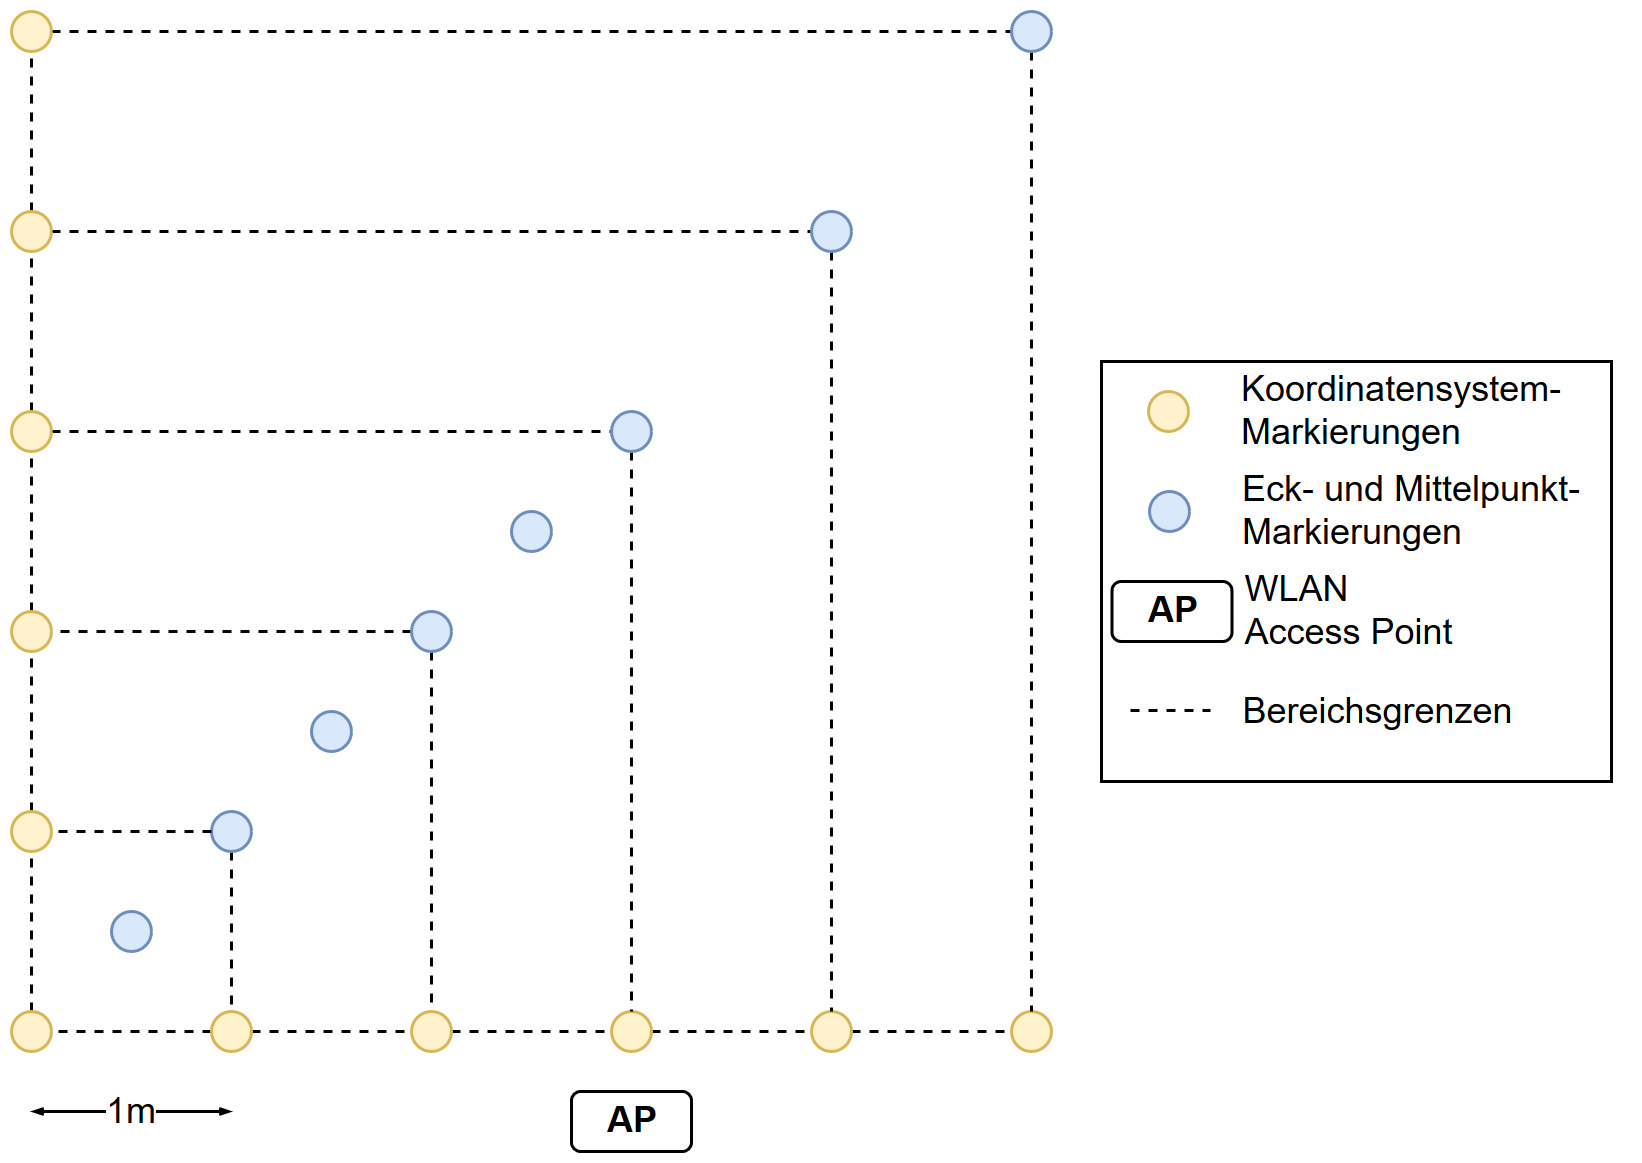
\includegraphics[scale=0.25]{images/testaufbau_interpolationsgenauigkeit.jpg}
\caption{\label{img:accuracy}Testaufbau zum Testen der Genauigkeit der Interpolation (Aufsicht)}
\end{figure}

Ein Testdurchlauf wurde nun durchgeführt, indem der Bereich der Messung auf das jeweilige Quadrat festgelegt wurde und an jedem der vier Eckpunkte je eine Messung durchgeführt wurde. Nun wurde die Heatmap generiert. Zur Auswertung der Interpolationsgenauigkeit bietet die App eine versteckte Debugging-Funktion: Tippt man nach Erstellung der Heatmap auf den Hilfetext am oberen Bildschirmrand (der zu diesem Zeitpunkt den Text \enquote{Heatmap erstellt} enthalten sollte), erhält man einen Toast mit der aktuell gemessenen WLAN-Empfangsfeldstärke und der Empfangsfeldstärke, die an der aktuellen Position in der Heatmap verzeichnet ist. Diese Funktion wurde zum Auswerten dieses Tests genutzt.

\begin{table}
\centering
\begin{tabular}{|r|r|r|r|r|r|}
\hline
Messung & Seitenlänge & RSSI interpoliert & RSSI gemessen & Abweichung & $\overline{x}_{Abweichung}$\\
Nr. & Fläche $[m]$ & $[dBm]$ & $[dBm]$ & $[dBm]$ & $[dBm]$\\\hline

1 & 1 & -45,15 & -48 & 2,85 & \\
2 & 1 & -45,49 & -47 & 1,51 & \\
3 & 1 & -47,08 & -45 & 2,08 & \\
4 & 1 & -46,74 & -45 & 1,74 & 2,045 \\\hline

5 & 2 & -45,41 & -41 & 4,41 & \\
6 & 2 & -45,04 & -42 & 3,04 & \\
7 & 2 & -46,33 & -41 & 5,33 & \\
8 & 2 & -44,39 & -43 & 1,39 & 3,543 \\\hline

9 & 3 & -45,18 & -46 & 0,82 & \\
10 & 3 & -44,50 & -45 & 0,50 & \\
11 & 3 & -43,87 & -47 & 3,13 & \\
12 & 3 & -44,12 & -47 & 2,88 & 1,833 \\\hline

13 & 4 & -43,26 & -45 & 1,74 & \\
14 & 4 & -45,22 & -44 & 1,22 & \\
15 & 4 & -44,63 & -41 & 3,63 & \\
16 & 4 & -44,27 & -43 & 1,27 & 1,965 \\\hline

17 & 5 & -46,49 & -45 & 1,49 & \\
18 & 5 & -48,08 & -46 & 2,08 & \\
19 & 5 & -47,56 & -48 & 0,44 & \\
20 & 5 & -44,81 & -46 & 1,19 & 1,300 \\\hline
\end{tabular}
\caption{\label{tab:interpolation}Testergebnisse: Genauigkeit der Interpolation.}
\end{table}

In der Tabelle \ref{tab:interpolation} sind die Ergebnisse dieses Tests zusammengefasst. Die Anzahl an Tests ist zu gering und die Messungenauigkeit (siehe Kapitel \ref{reproductability}) zu groß, um einen Zusammenhang zwischen Flächengröße und Interpolationsgenauigkeit festzustellen. Allerdings beträgt die durchschnittliche Ungenauigkeit der interpolierten Werte weniger als die mögliche Abweichung einer einzelnen Messung ($6,36$ dBm) und nur knapp mehr als die Standardabweichung ($1,478$ dBm) von RSSI-Messungen. Somit kann gesagt werden, dass sich die angewandte Interpolationsmethode unter Berücksichtigung der Ungenauigkeit der RSSI-Werte des Smartphones eignet, um die Lücken zwischen den Messpunkten zu füllen.

\subsection{Einfluss der Smartphonehaltung auf die Messung}
Bei der Vermessung mit der App können unterschiedliche Arten das Smartphone zu halten die Messung unterschiedlich beeinflussen. Dies sollte mit dem folgenden Test untersucht werden. Auch bei diesem Test ist das Ergebnis aus dem Test zu der Reproduzierbarkeit von Messungen (siehe Kapitel \ref{reproductability}) zu beachten, entsprechend kleine Unterschiede können auch auf die Inkonsistenz von Messwerten des Smartphones zurückzuführen sein.

Für diesen Test wurde ein vordefinierter Bereich von $4\cdot 4$ m als Bereich der Heatmap definiert. An den Eckpunkten des Bereichs wurden dann Messungen durchgeführt. Dabei wurde das Smartphone bei unterschiedlichen Durchläufen unterschiedlich gehalten.

\begin{table}
\centering
\begin{tabular}{|r|r|r|r|r|r|}
\hline
Messung & Smartphone Winkel & & LOS & RSSI & Messung $-$ Messung A\\
ID & (zum Boden) $[^\circ]$ & Griff-Art & zum AP & $[dBm]$ & $[dBm]$\\\hline

A1 & & & & -49,55 & 0,00 \\
A2 & & & & -47,68 & 0,00 \\
A3 & & & & -42,46 & 0,00 \\
A4 & 0 & Ganze Hand & Ja & -34,69 & 0,00 \\\hline

B1 & & & & -48,69 & 0,86 \\
B2 & & & & -48,78 & -1,10 \\
B3 & & & & -44,53 & -2,07 \\
B4 & 0 & Fingerspitzen & Ja & -38,57 & -3,88 \\\hline

C1 & & & & -46,00 & 3,55 \\
C2 & & & & -43,95 & 3,73 \\
C3 & & & & -46,33 & -3,87 \\
C4 & 90 & Fingerspitzen & Ja & -34,59 & 0,10 \\\hline

D1 & & & & -50,00 & -0,45 \\
D2 & & & & -46,53 & 1,15 \\
D3 & & & & -44,00 & -1,54 \\
D4 & 45 & Fingerspitzen & Ja & -38,17 & -3,48 \\\hline

E1 & & & & -48,38 & 1,17 \\
E2 & & & & -47,57 & 0,11 \\
E3 & & & & -45,37 & -2,91 \\
E4 & 0 & Fingerspitzen & Nein & -36,36 & -1,67 \\\hline

\end{tabular}
\caption{\label{tab:smartphonepose}Testergebnisse: Einfluss der Smartphonehaltung}
\end{table}

In Tabelle \ref{tab:smartphonepose} sieht man die Ergebnisse der Testdurchläufe. Es fällt zunächst auf, dass das Halten des Smartphones an den Fingerspitzen keine Verbesserung des RSSI bringt, eher im Gegenteil. Dies lässt sich auf die Antennenposition im verwendeten Testgerät (\textit{Google Pixel 2}) zurückführen. In dem Gerät befinden sich die WLAN-Antennen an der oberen Kante, sie liegen also bei beiden Griff-Arten frei. Des Weiteren kann den Daten entnommen werden, dass alle Messwerte (an den jeweiligen Punkten) innerhalb der in Kapitel \ref{reproductability} bestimmten, möglichen Abweichung und knapp über der Standardabweichung liegen. Daher spielt es für die Bestimmung von Orten mit schwachem WLAN-Empfang keine Rolle, ob bei der Messung das Smartphone in die Richtung des AP oder von ihm weg (also mit einer Person dazwischen) gehalten wird. Auch die Griff-Art hat keinen signifikanten Einfluss, solange die WLAN-Antenne nicht verdeckt wird. Beim Winkel des Smartphones kann erkannt werden, dass ein $90^\circ$-Winkel zum Boden einen geringfügig besseren Empfang liefern kann. Diese Verbesserung liegt aber ebenfalls in einem so kleinen Bereich (maximal $3,73$ dBm), dass sie als nicht relevant zur Bestimmung von schlecht versorgten Bereichen angesehen werden kann. Die Haltung des Smartphones ist also unter Berücksichtigung der ohnehin vorhandenen Ungenauigkeit der Messung nicht relevant, um Bereiche mit schlechtem WLAN-Empfang zu identifizieren.

\subsection{ARCore Genauigkeit}
\label{arcoreaccuracytest}
Die Untersuchung der Genauigkeit der Positionierung von ARCore gestaltete sich als besonders schwierig. Dies lag zum einen an der Verschlossenheit des Frameworks, zum anderen an der starken Abhängigkeit von der Umgebung. Unterschiedliche Lichtverhälnisse, Farben und Texturen der Umgebung können die Genauigkeit stark beeinflussen. Als Testumgebung für diese Tests wurde ebenfalls die WLAN-Teststrecke der AVM GmbH gewählt, die mit Sonnenlicht durch Milchglasfenster beleuchtet wurde. Die Umgebung war ausreichend mit leicht unterscheidbaren Objekten mit verschiedenen Farben (gelbe Säulen, roter Boden mit gelben Linien an Säulenpositionen sowie viele Akzentfarben) ausgestattet. So wurde eine erkennungsfreundliche Umgebung für diese Tests genutzt. Daher können Tests in ungünstigeren Umgebungen deutlich andere Ergebnisse liefern. Die an dieser Stelle durchgeführten Tests liefern lediglich Werte für günstige Umgebungen.

In diesen Tests sollten zwei Größen untersucht werden: Die Ungenauigkeit bei der Positionierung von entfernten Punkten und die Nachkorrektur der Position von Punkten, nachdem sich von diesem Punkt entfernt wurde.

\subsubsection{Punkt in großer Entfernung platzieren}
Um die Genauigkeit bei der Platzierung von Objekten in einiger Entfernung zu testen, wurde eine Startposition gewählt, von der aus die App gestartet wird. Außerdem wurde eine Zielposition gewählt, an der ein kariertes Blatt Papier platziert wurde. In der Mitte des Papiers wurde der Zielpunkt mit einem Stift markiert. Nun wurde die App am Startpunkt gestartet. Je nach Durchlauf wurden dann entsprechende Bewegungen (leichtes Kreisen der Hand, Absenken des Smartphones auf den Boden, Ablaufen der Strecke) durchgeführt, um der Umgebungserkennung viele oder wenige Daten zur Verfügung zu stellen. Nun wurde der Startpunkt\footnote{Hierbei handelte es sich um den Startpunkt zur Markierung des Heatmap-Bereiches.} auf der Startposition platziert und ein weiterer Bereichspunkt am Zielpunkt. An letzterem Punkt wurden nun die Messungen durchgeführt. Mithilfe der AR-Ansicht wurde bestimmt, an welcher Stelle sich der Punkt auf dem Boden befindet und wie weit er vom Zielpunkt entfernt war. Hierzu musste senkrecht auf den Punkt geblickt werden, um die exakte Position auf dem Boden zu bestimmen. Diese Position wurde auf dem Blatt Papier markiert. Zur Bestimmung der Höhe konnte nur mit einem Maßband und der AR-Ansicht von der Seite gearbeitet werden. Die Unterseite der blauen Säule markiert die Position des virtuellen Punktes. Zur Bestimmung der Höhe des virtuellen Punktes über dem Boden wurde das Maßband auf den auf dem Blatt markierten Punkt gesetzt und der Abstand zur Unterseite der Säule gemessen. War die Säule im Boden, musste bis zur Oberseite gemessen werden. Von diesem Wert wurde dann die Höhe der Säule (20 cm) abgezogen. Auf diese Weise wurde die negative Höhe gemessen. Der Abstand auf dem Boden (Abstand des Zielpunkt zum markierten Punkt) und die Höhendifferenz ergaben zusammen dann den Fehlervektor.

\begin{table}
\centering
\begin{tabular}{|r|r|r|r|r|}
\hline
Messung & Entfernung & Fehler bei minimaler & Fehler bei flacher & Fehler bei Ablaufen \\
ID & $[m]$ & Bewegung $[m]$ & Perspektive $[m]$ & der Strecke $[m]$ \\\hline

A1 & & 0,01 & 0,00 & 0,00 \\
A2 & & 0,00 & 0,00 & 0,00 \\
A3 & & 0,00 & 0,00 & 0,01 \\
A4 & 1 & 0,01 & 0,00 & 0,00 \\\hline

B1 & & 0,04 & 0,01 & 0,02 \\
B2 & & 0,03 & 0,02 & 0,00 \\
B3 & & 0,01 & 0,05 & 0,01 \\
B4 & 5 & 0,06 & 0,00 & 0,01 \\\hline

C1 & & 0,11 & 0,05 & 0,02 \\
C2 & & 0,03 & 0,13 & 0,04 \\
C3 & & 0,09 & 0,04 & 0,03 \\
C4 & 10 & 0,07 & 0,06 & 0,03 \\\hline

D1 & & 0,13 & 0,20 & 0,08 \\
D2 & & 0,16 & 0,14 & 0,11 \\
D3 & & 0,09 & 0,18 & 0,05 \\
D4 & 20 & 0,22 & 0,16 & 0,01 \\\hline

\end{tabular}
\caption{\label{tab:araccuracy1}Testergebnisse: Genauigkeit Platzierung von Objekten}
\end{table}

In der Tabelle \ref{tab:araccuracy1} sind die Messergebnisse aus der Genauigkeitsmessung zur Platzierung von entfernten Punkten aufgetragen. Diese Tests sollten untersuchen, wie gut ARCore zusammengehörige Flächen bei unterschiedlich viel Informationen erkennen kann. Bei großer Differenz wurde die Fläche unter dem entfernten Punkt seperat von der Fläche des Startpunktes getrackt und anders als diese korrigiert. Bei einer geringen Abweichung wurden die entfernte Fläche und die Fläche unter dem Startpunkt entweder in gleichem Maße korrigiert oder als eine Fläche erkannt.

Es wurden drei verschiedene Datensammlungsmethoden getestet: Bei der ersten wird die kleinstmögliche Bewegung, die zur Erkennung des Bodens notwendig ist, durchgeführt; bei der zweiten Datensammlungsmethode wird nach Erkennen der ersten Fläche (in diesem Fall des Bodens) das Smartphone auf Bodenhöhe gebracht, sodass es eine Perspektive entlang des Bodens bekommt; bei der letzten Datensammlungsmethode wird die Strecke nach dem Erkennen des Bodens abgelaufen, bevor Punkte platziert werden. Besonders letztere Lösung erwies sich auf größere Distanzen wie 10m oder 20m als sehr effizient\footnote{Auf der Distanz von 20m war der Punkt schwer zu platzieren, die Ungenauigkeit des Punktes ist unter Umständen durch nicht genaues Zielen bedingt.}. ARCore erhält durch ein vorheriges Ablaufen ein gutes Bild der Umgebung und kann den Punkten sicher Orte zuweisen. Die Punkte werden hierbei maximal 11cm verschoben, eine Strecke die für WLAN-Empfang keine signifikante Rolle spielt.

Es gilt hierbei auch zu bedenken, dass bei den letzten Messungen der Punkt aus sehr großer Entfernung platziert wurde. Wenn der Bereich in der Praxisnutzung der App abgelaufen wird, ist die Distanz zu dem zu platzierenden Punkt deutlich geringer als 10m wenn nicht sogar geringer als 5m. ARCore funktioniert bei Distanzen $<5$m sehr genau, die Fehler bleiben bei dieser Distanz sehr gering.

\subsubsection{Korrektur des Startpunkts}
Bei der Bereichsdefinition wird der Bereich meistens mit dem Smartphone umlaufen. Dabei ist es gut möglich, dass ARCore nie ein Gesamtbild des Bereiches oder während des Umlaufens nie eine Perspektive auf den Startpunkt bekommt. Das Framework muss also neue Fixpunkte erkennen und zur Positionsverfolgung nutzen, ohne diese in direktem örtlichen Bezug zu einem Anchor oder zum Nullpunkt des Koordinatensystems zu bekommen. Dabei kann es gut passieren, dass sich kleine Fehler summieren und zu einer Verschiebung des Startpunktes führen. Diese Verschiebung fällt dann auf, wenn man wieder den Startpunkt erreicht, um den Bereich zu schließen. Der Startpunkt ist dann unter Umständen verschoben und wird, sobald er ins Bild kommt, wieder auf die korrekte Position korrigiert. Diese Korrektur ist zu schnell, um gemessen zu werden, sie kann jedoch mit einer Bildschirmaufnahme-Software aufgezeichnet werden. Mit einem karierten Blatt Papier unter dem Startpunkt lässt sich die Korrekturentfernung dann in der Aufnahme ablesen. Aufgrund dieses Vorgehens kann nur die horizontale Korrektur des Startpunktes bestimmt werden. Die vertikale Korrektur wird bei diesem Test vernachlässigt. Um möglichst gleichbleibende Bedingungen bei jedem Test zu gewährleisten, wurde das Smartphone für die gesamte Dauer des Tests mit der Kamera senkrecht in Richtung Boden gehalten.

\begin{table}
\centering
\begin{tabular}{|r|r|r|r|r|}
\hline
Messung & Untersuchte & horizontale & Fehler vor & Fehler nach \\
ID & Fläche & Korrektur $[m]$ & Korrektur $[m]$ & Korrektur $[m]$ \\\hline

A1 & & 0,01 & 0,01 & 0,00 \\
A2 & & 0,00 & 0,00 & 0,00 \\
A3 & & 0,02 & 0,01 & 0,01 \\
A4 & $1m \cdot 1m$ & 0,00 & 0,00 & 0,00 \\\hline

B1 & & 0,00 & 0,00 & 0,00 \\
B2 & & 0,00 & 0,02 & 0,02 \\
B3 & & 0,02 & 0,02 & 0,00 \\
B4 & $5m \cdot 5m$ & 0,00 & 0,01 & 0,01 \\\hline

C1 & & 0,03 & 0,05 & 0,02 \\
C2 & & 0,00 & 0,02 & 0,02 \\
C3 & & 0,02 & 0,02 & 0,00 \\
C4 & $8m \cdot 8m$ & 0,00 & 0,00 & 0,00 \\\hline

D1 & & 0,04 & 0,04 & 0,01 \\
D2 & & 0,05 & 0,05 & 0,00 \\
D3 & & 0,03 & 0,02 & 0,01 \\
D4 & $10m \cdot 10m$ & 0,00 & 0,04 & 0,04 \\\hline

E1 & & 0,07 & 0,04 & 0,03 \\
E2 & & 0,00 & 0,01 & 0,01 \\
E3 & & 0,12 & 0,13 & 0,02 \\
E4 & $20m \cdot 2m$ & 0,04 & 0,09 & 0,06 \\\hline

\end{tabular}
\caption{\label{tab:araccuracy2}Testergebnisse: Korrektur des Startpunkts}
\end{table}

Aus den Testergebnissen (siehe Tabelle \ref{tab:araccuracy2}) kann zunächst entnommen werden, dass die Korrektur nicht immer in die richtige Richtung erfolgt ist. Zieht man die Korrektur von der Fehlerdistanz ab, erhält man nicht immer die exakte Fehlerdistanz nach der Korrektur. Daher wurde an einigen Stellen nur in die annähernd korrekte Richtung korrigiert.

Den Ergebnissen kann außerdem entnommen werden, dass der Fehler - beziehungsweise die Größe der notwendigen Korrektur - nicht von der Fläche des abgelaufenen Bereiches abhängt, sondern eher von der größten Entfernung vom Startpunkt. Die Tests D und E haben die gleiche Fläche während sich in Test E deutlich weiter von Startpunkt entfernt wird. Der Fehler des Startpunktes für Tests in E ist dementsprechend im Durchschnitt größer.

Die Fehler nach der Korrektur fallen für die getesteten Flächen gering genug aus, um eine Positionierung von WLAN Messungen und ein genaues Platzieren der Heatmap auf dem Boden zu ermöglichen. Größere Flächen sind an dieser Stelle nicht getestet worden, da Lichtverhältnisse und andere Einflüsse bei größeren Bereichen schnell zu einem komplettem Positionsverlust führen können. Die Fläche von $20m \cdot 2m$ war die größte Fläche, bei der bei vier Tests kein Positionsverlust vorgekommen ist. Es gilt hierbei jedoch zu beachten, dass dies stark von der Umgebung und der Art, wie das Smartphone gehalten wird (nur Boden im Sichtfeld der Kamera oder der gesamte Raum), abhängt.

Bei diesem großflächigen Test ist ebenfalls aufgefallen, dass die Heatmap ab einer hohen Anzahl an Pixeln kleiner skaliert wird und nicht mehr korrekt im Vergleich zum definierten Bereich skaliert. Bei weiteren kleinen Tests zu diesem Thema konnte erkannt werden, dass eine Erhöhung der Heatmap-Auflösung diesen Effekt bei kleineren Flächen hervorruft und durch Verringern der Auflösung eine deutlich größere Fläche analysiert werden kann, bevor der Effekt erneut auftritt. Der Fehler ist also durch die Pixelanzahl und nicht die Größe der Heatmap bedingt. Vermutlich handelt es sich hierbei um einen Fehler in ARCore oder Sceneform. Um dem entgegen zu wirken, kann man für Flächen größer als $10m \cdot 10m$ die Auflösung der Heatmap von den standardmäßig eingestellten 100 Pixeln pro Meter auf 10 Pixel reduzieren. 

\subsection{Realisierbarkeit Abstandsmessung mithilfe von 802.11mc}
\label{RTTTest}
In dieser Arbeit wurde auch untersucht, in welchem Rahmen das neue RTT-Verfahren des 802.11mc WLAN-Standards zur Abstandsbestimmung zu einem AP geeignet ist. Mit diesem Abstand könnte eines der vorgestellten Ausbreitungsmodelle angewandt werden um nicht interpolierbare Werte zu extrapolieren. Hierfür wurde eine kleine Demo-App (RTT Demo, siehe Kapitel \ref{rttapp}) geschrieben und eine \textit{FRITZ!Box 7590} mit einer speziell modifizierten Firmware verwendet. Diese Tests ergaben extreme Abweichungen ($> 10$m, siehe Tabelle \ref{tab:rtt}) von der tatsächlichen Distanz. Dies ist dadurch bedingt, dass ein Router, der das RTT-Verfahren unterstützen soll, eine sehr genau kalibrierte Uhr benötigt. Eine solche Genauigkeit ist bisher für keinen Anwendungsfall notwendig gewesen. Dementsprechend ist bestehende Hardware nicht auf den Einsatz vom RTT-Verfahren vorbereitet und liefert diese starken Abweichungen. Erst mit speziell ausgelegter Hardware wird eine Entfernungsbestimmung mithilfe von RTT umsetzbar. Aufgrund des Ergebnisses von diesem Test wurde die Extrapolation in dem in dieser Arbeit erstelltem Prototyp nicht umgesetzt. Zukünftige Hardware bietet unter Umständen eine bessere Genauigkeit, wodurch dieser Ansatz umsetzbar wird.

\begin{table}
\centering
\begin{tabular}{|r|r|r|r|r|r|r|}
\hline
Messung & 1 & 2 & 3 & 4 & 5 & 6 \\\hline
gemessener Abstand $[m]$ & -1,34 & -2,56 & -3,38 & -0,74 & -2,88 & -4,73\\
\hline
\end{tabular}
\caption{\label{tab:rtt}Testergebnisse: RTT Distanz (Smartphone war 10m vom AP entfernt)}
\end{table}

\section{Fazit}
Im Rahmen dieser Arbeit wurde eine Android-App erstellt, mit der es möglich ist die WLAN-Empfangsstärke zu analysieren. Der entwickelte Prototyp ist in der Lage die WLAN-Verteilung innerhalb von Räumen zuverlässig darzustellen. Das Framework ARCore eignet sich dabei sehr gut zur Positionierung von Messungen, als Eingabemethode für Bereiche und zur Darstellung der Ergebnisse. Die Genauigkeit des Frameworks ist für einzelne Räume und bei sehr guten Umgebungsverhältnissen für ganze Etagen ausreichend. 

Die App bietet vielfältige Einstellungen zur Anpassung der Analyse. So können die Farben, die Auflösung und weitere Parameter der Heatmap verändert werden, um das Ergebnis nach Wunsch anzupassen. Die Darstellung der Heatmap in AR erlaubt es dem Nutzer das Ergebnis zu begehen und ermöglicht eine realitätsnähere Visualisierung der Verteilung des WLAN-Signals als eine Karte dies könnte.

Um mehrere Messungen zu vergleichen, oder die Ergebnisse jemandem zu schicken, kann die Heatmap als Bild im Speicher des Smartphones abgelegt werden. Die Heatmap kann dabei nach Wunsch gedreht werden um sie in der gewünschten Orientierung zu speichern.

Der Prototyp erfüllt damit alle in der Anforderungsanalyse spezifizierten erforderliche Kriterien. Die Position des Android-Geräts kann relativ zu der Position, an der die App gestartet wurde - und somit relativ zur Umgebung - verfolgt werden. Nach dem Start der App kann der Bereich, in dem die Heatmap gezeichnet werden soll, mithilfe von AR definiert werden. AR eignet sich hier gut als intuitive Eingabemethode. Die Abweichung von AR im Vergleich zu den tatsächlichen Positionen befindet sich dabei mit günstigen Umgebungsverhältnissen unter 10cm. Beim Vermessen der Empfangsstärke in der Umgebung kann jeder Messung mithilfe von ARCore eine Position relativ zum Bereich zugewiesen werden, solange ARCore in der Lage ist, genug Fixpunkte in der Umgebung zu erkennen. Aus diesen Messpunkten kann im Anschluss eine vollständige Heatmap generiert werden. Zwischen den Messpunkten wird dabei interpoliert und die interpolierten Empfangsstärken sind dabei nah an gemessenen Werten. Werte, die nicht durch Interpolation bestimmt werden können verfolgen den Nearest-Neighbor-Ansatz und nehmen den Wert des räumlich nächsten Messpunkts an.

Auch einige optionale Anforderungen konnten umgesetzt werden. So ist die Ortung mit ARCore deutlich genauer als ursprünglich erwartet. Die Heatmap kann deshalb sehr gut in AR dargestellt werden, um das Ergebnis begehbar zu machen. Die Einstellung \enquote{Farbverlauf Breite} erlaubt außerdem entweder eine Heatmap mit fließenden Übergängen oder eine mit \enquote{Zonen} zu generieren. So kann die Analyse der WLAN-Empfangsstärke in klassifizierten Bereichen erfolgen. Auch die Auflösung der Heatmap ist verstellbar. Die optionale Anforderung, nicht interpolierbare Werte durch Extrapolation mithilfe eines Ausbreitungsmodells zu bestimmen, konnte hingegen nicht umgesetzt werden. Dies ist zum einen durch den zeitlichen Rahmen dieser Arbeit, zum anderen durch mangelnde Vorbereitung von Hardware für das RTT-Verfahren bedingt. Sollte es in Zukunft möglich sein, den Abstand zu einem AP genauer zu bestimmen, würde die Extrapolation in dieser App umsetzbar werden.

Dieser Prototyp könnte in Zukunft als Grundlage für eine Endanwender-orientierte App zur WLAN-Analyse dienen. Hierzu könnte man anstatt der Empfangsstärke zum Beispiel die Verbindungsgeschwindigkeit messen, um die tatsächliche Auswirkung auf die Nutzung des Smartphones zu bestimmen. Das Laden und anschließende Platzieren alter Heatmaps in AR würde die Analyse von Bereichen erlauben, bei denen ARCore aufgrund der Größe oder schweren Umgebung die Position nicht durchgängig verfolgen kann. Auch eine Unterscheidung zwischen verschiedenen APs und den unterschiedlichen Bändern wäre bei einer solchen App von Nutzen, sowie automatische Empfehlungen für die Platzierung des APs oder von Repeatern.


%Performance: Triangulation bei Messung

%2,4 und 5 Band

%Mehr Einfärbungsmethoden -> Farbenblind (mehr farben)

%Durchsatz anstatt RSSI

%Mehr Dimensionen (Treppen etc.)

%RTT zur Extrapolation und/oder Positionsbestimmung Router

%Manuelles Setzen von Farbgrenzen

%Laden und Platzieren alter Heatmaps

%Farbverlauf mit Signal Level

%Mehr fläche analysieren


% ### END ###
\cleardoublepage

\section{Literaturverzeichnis}
\begingroup
% Disable the section command for the bibliography to prevent it from generating its own header
\renewcommand{\section}[2]{}
\printbibliography
\endgroup

\section{Abkürzungsverzeichnis}
\begin{tabular}{ll}
\textbf{AP:} & Access Point\\
\textbf{AR:} & Augmented Reality\\
\textbf{IDE:} & Integrated Development Environment\\
\textbf{LOS:} & Line of sight\\
\textbf{MVC:} & Model View Controller\\
\textbf{RTT:} & Round-Trip-Time\\
\textbf{TOF:} & Time of flight\\
\textbf{UI:} & User Interface\\
\textbf{WLAN:} & Wireless Local Area Network\\
\textbf{HMD:} & Head-Mounted-Display\\
\end{tabular}

\section{Abbildungsverzeichnis}
\begingroup
% Disable the section command for the figure list to prevent it from generating its own header
\renewcommand{\section}[2]{}
\listoffigures
\endgroup

\section{Tabellenverzeichnis}
\begingroup
% Disable the section command for the table list to prevent it from generating its own header
\renewcommand{\section}[2]{}
\listoftables
\endgroup
\newpage
\section{Glossar}
\textbf{Access Point:} Ein WLAN Zugangspunkt. Dieser stellt ein WLAN-Netz zur Verfügung.\\~\\
\textbf{Anchor:} Eine Klasse aus dem Framework ARCore die einen virtuellen Anker repräsentiert. Dieser Anker bleibt immer am gleichen Ort, da er an eine Oberfläche gebunden wird.\\~\\
\textbf{Android-App:} Eine Anwendung, die auf einem Android-Gerät lauffähig ist und für ein solches entwickelt wurde.\\~\\
\textbf{AR-Umgebung:} Bezeichnet die Kombination aus der realen Umgebung und der virtuellen.\\~\\
\textbf{ARCore:} Ein Framework von Google Inc. zum Erstellen von Augmented Reality Apps. Es bringt Funktionen zur Bewegungserkennung, Umgebungserkennung (Erkennen von Objekten oder Flächen) und zum Erkennen von Lichtverhältnissen.\\~\\
\textbf{Button:} Die Bezeichnung für eine Schaltfläche in Android.\\~\\
\textbf{Button-Bar:} Die Bezeichnung für eine Leiste mit Schaltfläche in Android.\\~\\
\textbf{Heatmap:} Eine zweidimensionale Karte, auf der die WLAN-Empfangsfeldstärke farblich gekennzeichnet wird.\\~\\
\textbf{Konvexe Hülle:} Ein Polygon, das eine Menge von Punkten so einschließt, dass keine Verbindungsstrecke zwischen zwei Punkten der Punktemenge außerhalb dieser Figur liegt.\\~\\
\textbf{Minimal umgebendes Rechteck (auch minimal umschließendes Rechteck):} Das kleinstmögliche (kleinste Fläche) Rechteck, dessen Seiten parallel zu den x- und y-Achsen eines 2D-Koordinatensystems verlaufen, welches eine Form, eine Menge von Formen oder eine Menge von Punkten einschließt.\\~\\
\textbf{Plane:} Eine Klasse aus dem Framework ARCore, die eine erkannte Ebene repräsentiert.\\~\\
\textbf{QR-Code:} Quick-Response Code, Verfahren zur optischen Übertragung von Informationen\\~\\
\textbf{Received Signal Stregth:} Die gemessene Energie auf der Empfängerseite einer Funkverbindung.\\~\\
\textbf{Received Signal Stregth Indicator:} Ein Indikator für die gemessene Energie auf der Empfängerseite einer Funkverbindung. Gängige Einheiten sind $dBm$, $mW$ oder Signallevel wie zum Beispiel die Anzeige für WLAN-Empfang auf Smartphones.\\~\\
\textbf{ScanResults:} Ergebnisse eines durch das Android Betriebssystem durchgeführten WLAN-Scans.\\~\\
\textbf{Sceneform:} Ein Framework von Google Inc. zum Erstellen von 3D-Objekten und zum Platzieren jener Objekte in Augmented Reality mit ARCore. Sceneform erlaubt die Nutzung von ARCore ohne OpenGL-Kenntnisse.\\~\\
\textbf{Tap Target:} Bezeichnet eine besondere Art der Hilfestellung, bei der die Funktion eines Knopfes erläutert wird. Hierzu wird der Knopf besonders hervorgehoben und ein Hilfetext sehr prominent (vor anderen Bedienelementen) dazu angezeigt.\\~\\
\textbf{Toast:} Bezeichnet im Kontext dieser Arbeit einen auf Android-Geräten über der Obfläche, sehr prominent angezeigten Text.\\~\\
\textbf{ToF-Kamera:} Eine 3D-Kamera, die mit dem Laufzeitverfahren (engl. time of flight) Entfernungen bestimmen kann. Der Vorteil dieser Technologie ist, dass die Szene nicht abgetastet werden muss sondern auf einmal aufgenommen wird.\\~\\
\textbf{Triangulation:} Mit Triangulation wird in dieser Arbeit das Aufteilen der konvexen Hülle einer Punktemenge in Dreiecke beschrieben, wobei die Eckpunktmenge von den Dreiecken genau die Punktmenge ist.\\~\\
\textbf{Wertematrix:} Ein zweidimensionaler Array mit dem Datentyp Double.\\~\\

\newpage
\section*{Eigenständigkeitserklärung}
Hiermit versichere ich, dass ich die vorliegende Bachelorarbeit selbstständig und nur unter Verwendung der angegebenen Quellen und Hilfsmittel verfasst habe. Die Arbeit wurde bisher in gleicher oder ähnlicher Form keiner anderen Prüfungsbehörde vorgelegt.

\vskip 1cm

Berlin, den 13. August 2018

\vskip 1.5cm

Emil Schoenawa
\end{document}
